% =====================================================================
%  PAPER IV -- When the Attacker Is Indistinguishable from the Weather
%  Target: IEEE Symposium on Security and Privacy (double-blind).
%  Format: IEEEtran, conference mode, letter paper, 10 pt, two columns;
%  body within 13 pages, references and appendices excluded.
%    latexmk -pdf main.tex      (pdfLaTeX + BibTeX)
%  Every number is a macro from numbers.tex (generated by
%  ../experiments/make_numbers.py). Never type a result into this file.
% =====================================================================
\documentclass[conference,letterpaper,10pt]{IEEEtran}
\IEEEoverridecommandlockouts
\usepackage{mathptmx}
\usepackage[T1]{fontenc}
\usepackage[scaled=0.92]{helvet}   % scalable sans (TikZ labels)
\usepackage{courier}               % scalable typewriter (provenance flags)
\usepackage[utf8]{inputenc}
\usepackage{amsmath,amssymb,amsthm,mathtools}
\usepackage{cite}
\usepackage{booktabs,multirow,array,tabularx,colortbl}
\usepackage{graphicx,xcolor}
\usepackage{tikz,pgfplots}
\usetikzlibrary{positioning,arrows.meta,fit,backgrounds,calc,shapes.geometric}
\pgfplotsset{compat=1.17}
\usepackage[hidelinks]{hyperref}
\usepackage[capitalize,nameinlink]{cleveref}
\usepackage{enumitem}
\setlist{leftmargin=1.2em,itemsep=1pt,topsep=2pt}
\usepackage{microtype}
\setlength{\emergencystretch}{1.5em}

% ---------------- colours (colour-blind-safe palette) ----------------
\definecolor{cBlue}{HTML}{2C6E9B}
\definecolor{cGreen}{HTML}{3B8B5A}
\definecolor{cOrange}{HTML}{C77D1A}
\definecolor{cRed}{HTML}{B03A2E}
\definecolor{cPurple}{HTML}{6A4C93}
\definecolor{cGray}{HTML}{555555}

% ---------------- notation ---------------------------------------------
\newcommand{\dnet}{\delta_{\mathrm{net}}}
\newcommand{\dfault}{\delta_{\mathrm{fault}}}
\newcommand{\denv}{\delta_{\mathrm{env}}}
\newcommand{\dgnss}{\delta_{\mathrm{gnss}}}
\newcommand{\dadv}{\delta_{\mathrm{adv}}}
\newcommand{\dtot}{\delta_{\mathrm{tot}}}
\newcommand{\TV}{\mathrm{TV}}
\newcommand{\KL}{\mathrm{KL}}
\newcommand{\MCR}{\mathrm{MCR}}
\newcommand{\Fbar}{\overline{F}}
\newcommand{\pbar}{\overline{p}}
\newcommand{\E}{\mathbb{E}}
\newcommand{\R}{\mathbb{R}}
\newcommand{\Dclass}{\mathcal{D}}
\newcommand{\code}[1]{\texttt{\small #1}}
\newtheorem{definition}{Definition}
\newtheorem{lemma}{Lemma}
\newtheorem{proposition}{Proposition}
\newtheorem{theorem}{Theorem}
\newtheorem{corollary}{Corollary}
\theoremstyle{remark}
\newtheorem{remark}{Remark}

% Generated by experiments/make_numbers.py -- do not edit by hand.
\newcommand{\nAmp}{3.26}
\newcommand{\nAnchorArgFive}{gnss mimic}
\newcommand{\nAnchorArgTen}{fault mimic}
\newcommand{\nAnchorArgTwenty}{step}
\newcommand{\nAnchorMaxFive}{4.4}
\newcommand{\nAnchorMaxTen}{9.0}
\newcommand{\nAnchorMaxTwenty}{20.6}
\newcommand{\nAnchorMultTwenty}{4.7}
\newcommand{\nBenignNoAlarm}{94\%}
\newcommand{\nBestALLDev}{2.9}
\newcommand{\nBestALLFam}{weather mimic}
\newcommand{\nBestDFourDev}{2.9}
\newcommand{\nBestDFourFam}{weather mimic}
\newcommand{\nBestDOneDev}{2.9}
\newcommand{\nBestDOneFam}{weather mimic}
\newcommand{\nBestDThreeDev}{2.8}
\newcommand{\nBestDThreeFam}{weather mimic}
\newcommand{\nBestDTwoDev}{2.9}
\newcommand{\nBestDTwoFam}{weather mimic}
\newcommand{\nCalMissions}{4{,}000}
\newcommand{\nCells}{25}
\newcommand{\nCemGens}{25}
\newcommand{\nCemK}{48}
\newcommand{\nCrossEvMin}{87\%}
\newcommand{\nCrossEvMinAll}{88\%}
\newcommand{\nDadvArgFive}{fault mimic}
\newcommand{\nDadvArgOne}{fault mimic}
\newcommand{\nDadvArgTen}{fault mimic}
\newcommand{\nDadvFive}{4.37}
\newcommand{\nDadvOne}{4.37}
\newcommand{\nDadvTen}{4.37}
\newcommand{\nDepRatio}{4}
\newcommand{\nDevALLFaultMimic}{2.6}
\newcommand{\nDevALLGnssMimic}{2.5}
\newcommand{\nDevALLRamp}{2.4}
\newcommand{\nDevALLStep}{2.1}
\newcommand{\nDevALLWeatherMimic}{2.9}
\newcommand{\nDevAllMax}{2.9}
\newcommand{\nDevAllMin}{2.1}
\newcommand{\nDevDFourFaultMimic}{2.6}
\newcommand{\nDevDFourGnssMimic}{2.5}
\newcommand{\nDevDFourRamp}{2.4}
\newcommand{\nDevDFourStep}{2.1}
\newcommand{\nDevDFourWeatherMimic}{2.9}
\newcommand{\nDevDOneFaultMimic}{2.6}
\newcommand{\nDevDOneGnssMimic}{2.5}
\newcommand{\nDevDOneRamp}{2.4}
\newcommand{\nDevDOneStep}{2.1}
\newcommand{\nDevDOneWeatherMimic}{2.9}
\newcommand{\nDevDThreeFaultMimic}{2.6}
\newcommand{\nDevDThreeGnssMimic}{2.5}
\newcommand{\nDevDThreeRamp}{2.4}
\newcommand{\nDevDThreeStep}{2.1}
\newcommand{\nDevDThreeWeatherMimic}{2.8}
\newcommand{\nDevDTwoFaultMimic}{2.6}
\newcommand{\nDevDTwoGnssMimic}{2.5}
\newcommand{\nDevDTwoRamp}{2.4}
\newcommand{\nDevDTwoStep}{2.1}
\newcommand{\nDevDTwoWeatherMimic}{2.9}
\newcommand{\nDevSingleMax}{2.9}
\newcommand{\nDevSingleMin}{2.1}
\newcommand{\nDiagAllSat}{all}
\newcommand{\nDiagAttackMax}{2.3}
\newcommand{\nDiagBenignMax}{34.5}
\newcommand{\nDiagBenignMin}{19.2}
\newcommand{\nDiagMissions}{3}
\newcommand{\nEnvRatio}{2.2}
\newcommand{\nEvALLFaultMimic}{94\%}
\newcommand{\nEvALLGnssMimic}{91\%}
\newcommand{\nEvALLRamp}{90\%}
\newcommand{\nEvALLStep}{88\%}
\newcommand{\nEvALLWeatherMimic}{90\%}
\newcommand{\nEvDFourFaultMimic}{92\%}
\newcommand{\nEvDFourGnssMimic}{91\%}
\newcommand{\nEvDFourRamp}{90\%}
\newcommand{\nEvDFourStep}{87\%}
\newcommand{\nEvDFourWeatherMimic}{89\%}
\newcommand{\nEvDOneFaultMimic}{94\%}
\newcommand{\nEvDOneGnssMimic}{92\%}
\newcommand{\nEvDOneRamp}{91\%}
\newcommand{\nEvDOneStep}{89\%}
\newcommand{\nEvDOneWeatherMimic}{88\%}
\newcommand{\nEvDThreeFaultMimic}{94\%}
\newcommand{\nEvDThreeGnssMimic}{90\%}
\newcommand{\nEvDThreeRamp}{89\%}
\newcommand{\nEvDThreeStep}{89\%}
\newcommand{\nEvDThreeWeatherMimic}{88\%}
\newcommand{\nEvDTwoFaultMimic}{93\%}
\newcommand{\nEvDTwoGnssMimic}{91\%}
\newcommand{\nEvDTwoRamp}{90\%}
\newcommand{\nEvDTwoStep}{88\%}
\newcommand{\nEvDTwoWeatherMimic}{88\%}
\newcommand{\nEvalMissions}{1{,}000}
\newcommand{\nEventsReal}{200{,}610}
\newcommand{\nEventsTotal}{431{,}773}
\newcommand{\nFprAnchor}{0.95\%}
\newcommand{\nFprGnssOnlyMax}{5.3\%}
\newcommand{\nFprModMax}{6.9\%}
\newcommand{\nFprModMin}{3.8\%}
\newcommand{\nFprSevereDThree}{8.2\%}
\newcommand{\nFprSevereOtherMax}{6.0\%}
\newcommand{\nFprWindFaultMax}{0.0\%}
\newcommand{\nGapIndep}{0.1223}
\newcommand{\nGapIndepMix}{0.0563}
\newcommand{\nGapJoint}{0.0031}
\newcommand{\nGapJointK}{62}
\newcommand{\nGapRa}{0.5133}
\newcommand{\nGapS}{4}
\newcommand{\nGapSumSame}{0.0515}
\newcommand{\nGapUnion}{0.6390}
\newcommand{\nGatedCap}{2.9}
\newcommand{\nGatedUnfFam}{weather mimic}
\newcommand{\nGatedUnfMax}{5.6}
\newcommand{\nGatedUnfStacks}{D1, D3}
\newcommand{\nHeldoutAdvFam}{fault mimic}
\newcommand{\nHeldoutAdvFpr}{5\%}
\newcommand{\nHeldoutAdvMax}{5.13}
\newcommand{\nHeldoutAdvRatio}{1.17}
\newcommand{\nJointMissions}{20{,}000}
\newcommand{\nKsCaughtMed}{0.99}
\newcommand{\nKsStealthyMed}{0.07}
\newcommand{\nMNinety}{10.0}
\newcommand{\nMNinetyIndep}{8.5}
\newcommand{\nMNinetyNet}{13.0}
\newcommand{\nMNinetyNine}{12.0}
\newcommand{\nMargEnvLoMax}{1.67}
\newcommand{\nMargEnvLoPnf}{1.11}
\newcommand{\nMargEnvMixMax}{3.06}
\newcommand{\nMargEnvMixPnf}{1.77}
\newcommand{\nMargEnvUpMax}{3.23}
\newcommand{\nMargEnvUpPnf}{2.17}
\newcommand{\nMargFaultMax}{2.28}
\newcommand{\nMargFaultPnf}{0.94}
\newcommand{\nMargGnssMax}{3.93}
\newcommand{\nMargGnssPnf}{2.27}
\newcommand{\nMargJointMax}{6.43}
\newcommand{\nMargJointPnf}{2.92}
\newcommand{\nMaxRateRatio}{0.00}
\newcommand{\nMissionsTotal}{1{,}909{,}600}
\newcommand{\nNatRatio}{1.09}
\newcommand{\nNegCfourMaxDev}{96.7}
\newcommand{\nNegCfourRows}{6}
\newcommand{\nNegCfourViol}{1}
\newcommand{\nNegCfourViolFam}{fault}
\newcommand{\nNegCtwoMaxDev}{308.5}
\newcommand{\nNegCtwoRows}{6}
\newcommand{\nNegCtwoViol}{4}
\newcommand{\nNegCtwoViolFam}{fault and ramp}
\newcommand{\nNetTubeQuarter}{2.65}
\newcommand{\nNgALLFaultMimic}{10.5}
\newcommand{\nNgALLGnssMimic}{2.6}
\newcommand{\nNgALLRamp}{2.4}
\newcommand{\nNgALLStep}{2.2}
\newcommand{\nNgALLWeatherMimic}{2.9}
\newcommand{\nNgArgALL}{fault mimic}
\newcommand{\nNgArgDFour}{fault mimic}
\newcommand{\nNgArgDOne}{fault mimic}
\newcommand{\nNgArgDThree}{fault mimic}
\newcommand{\nNgArgDTwo}{fault mimic}
\newcommand{\nNgCapALL}{10.5}
\newcommand{\nNgCapDFour}{73.9}
\newcommand{\nNgCapDOne}{73.9}
\newcommand{\nNgCapDThree}{73.9}
\newcommand{\nNgCapDTwo}{9.9}
\newcommand{\nNgDFourFaultMimic}{73.9}
\newcommand{\nNgDFourGnssMimic}{2.6}
\newcommand{\nNgDFourGnssUnf}{19.2}
\newcommand{\nNgDFourRamp}{2.4}
\newcommand{\nNgDFourStep}{2.2}
\newcommand{\nNgDFourWeatherMimic}{3.3}
\newcommand{\nNgDOneFaultMimic}{73.9}
\newcommand{\nNgDOneGnssMimic}{72.6}
\newcommand{\nNgDOneRamp}{2.4}
\newcommand{\nNgDOneStep}{2.2}
\newcommand{\nNgDOneWeatherMimic}{50.4}
\newcommand{\nNgDThreeFaultMimic}{73.9}
\newcommand{\nNgDThreeGnssMimic}{37.9}
\newcommand{\nNgDThreeRamp}{2.4}
\newcommand{\nNgDThreeStep}{2.2}
\newcommand{\nNgDThreeWeatherMimic}{37.2}
\newcommand{\nNgDTwoFaultMimic}{9.9}
\newcommand{\nNgDTwoGnssMimic}{2.6}
\newcommand{\nNgDTwoRamp}{2.4}
\newcommand{\nNgDTwoStep}{2.2}
\newcommand{\nNgDTwoUnfMax}{9.9}
\newcommand{\nNgDTwoWeatherMimic}{2.9}
\newcommand{\nNgEvMin}{94\%}
\newcommand{\nNgMax}{73.9}
\newcommand{\nNgStepUnfMax}{26.8}
\newcommand{\nOpenArgFive}{fault mimic}
\newcommand{\nOpenArgTen}{fault mimic}
\newcommand{\nOpenArgTwenty}{fault mimic}
\newcommand{\nOpenMaxFive}{8.3}
\newcommand{\nOpenMaxTen}{33.6}
\newcommand{\nOpenMaxTwenty}{137.8}
\newcommand{\nOpenMultTwenty}{17}
\newcommand{\nOpenRatioTwenty}{7}
\newcommand{\nOwnOptFail}{8}
\newcommand{\nParentGamma}{1.625}
\newcommand{\nParentHops}{15{,}392}
\newcommand{\nParentL}{1.181}
\newcommand{\nParentSlack}{4.84}
\newcommand{\nPooledAttackers}{35}
\newcommand{\nREightDOneFive}{303}
\newcommand{\nREightGateOnly}{unbounded}
\newcommand{\nREightSatFive}{31.9}
\newcommand{\nREightSatRatio}{5.8}
\newcommand{\nREightSatRatioAdv}{4.5}
\newcommand{\nRFiveEnvMax}{7.0}
\newcommand{\nRFiveEnvTen}{6.2}
\newcommand{\nRFiveFloorCpLong}{0.19}
\newcommand{\nRFiveFloorCpMeas}{0.21}
\newcommand{\nRFiveFloorCpSim}{0.54}
\newcommand{\nRFiveFloorCpTwenty}{0.992}
\newcommand{\nRFiveFloorLong}{0.32}
\newcommand{\nRFiveFloorMeas}{0.34}
\newcommand{\nRFiveFloorSim}{0.69}
\newcommand{\nRFivePnnMeas}{7.0}
\newcommand{\nRFivePnnSim}{2.8}
\newcommand{\nRFiveSamples}{496}
\newcommand{\nROneAdvMax}{7.04}
\newcommand{\nROneAdvMaxFam}{mixed}
\newcommand{\nROneAttackers}{126}
\newcommand{\nROneCells}{270}
\newcommand{\nROneCmaGens}{200}
\newcommand{\nROneCmaPop}{16}
\newcommand{\nROneDadvArg}{gnss mimic (tail-objective TPE)}
\newcommand{\nROneDadvFive}{5.46}
\newcommand{\nROneDadvOne}{5.46}
\newcommand{\nROneDadvRatioFive}{1.25}
\newcommand{\nROneDadvRatioOne}{1.25}
\newcommand{\nROneDadvRatioTen}{1.15}
\newcommand{\nROneDadvTen}{5.04}
\newcommand{\nROneEvalN}{5{,}000}
\newcommand{\nROneHeldSeeds}{5}
\newcommand{\nROneK}{128}
\newcommand{\nROnePerOpt}{42}
\newcommand{\nROneSupCem}{4.37}
\newcommand{\nROneSupCma}{3.85}
\newcommand{\nROneSupExceed}{12}
\newcommand{\nROneSupTpe}{3.09}
\newcommand{\nROneSupTpeTail}{5.46}
\newcommand{\nROneSuperposMin}{90.9\%}
\newcommand{\nROneTests}{1{,}620}
\newcommand{\nROneTrials}{400}
\newcommand{\nROneUndet}{797{,}435}
\newcommand{\nROneViol}{5}
\newcommand{\nROneViolM}{20}
\newcommand{\nROneViolPbarMax}{0.000}
\newcommand{\nRaGain}{20\%}
\newcommand{\nRevAdvMax}{6.25}
\newcommand{\nRevAdvMaxFam}{weather mimic}
\newcommand{\nRevAdvMaxOpt}{CEM}
\newcommand{\nRevAttackers}{72}
\newcommand{\nRevEmpCells}{216}
\newcommand{\nRevEmpExceed}{6}
\newcommand{\nRevEmpFailInf}{0}
\newcommand{\nRevEmpFloorTen}{0.541}
\newcommand{\nRevEmpFloorTwenty}{0.992}
\newcommand{\nRevEmpInformative}{648}
\newcommand{\nRevEmpMaxRatio}{0.00}
\newcommand{\nRevEmpTests}{1{,}296}
\newcommand{\nRevEmpViol}{0}
\newcommand{\nRevEmpWithin}{210}
\newcommand{\nRevFprSat}{5.6\%}
\newcommand{\nRevFprStack}{4.8\%}
\newcommand{\nRevGrid}{501}
\newcommand{\nRevLpCells}{216}
\newcommand{\nRevLpExceed}{0}
\newcommand{\nRevLpFailInf}{0}
\newcommand{\nRevLpFloorTen}{0.000}
\newcommand{\nRevLpFloorTwenty}{0.000}
\newcommand{\nRevLpInformative}{0}
\newcommand{\nRevLpMaxRatio}{--}
\newcommand{\nRevLpTests}{1{,}296}
\newcommand{\nRevLpViol}{0}
\newcommand{\nRevLpWithin}{216}
\newcommand{\nRevSatAlarmMax}{100.0\%}
\newcommand{\nRevSatAlone}{1.1\%}
\newcommand{\nRevSupUnsat}{0.0e+00}
\newcommand{\nRevUndet}{510{,}848}
\newcommand{\nRevZeroUndet}{25}
\newcommand{\nSatUnsatExcess}{7.8e-15}
\newcommand{\nSatUnsatMin}{100.00\%}
\newcommand{\nSoundNontrivial}{135}
\newcommand{\nSoundPoints}{270}
\newcommand{\nSoundViol}{0}
\newcommand{\nSoundViolIndep}{0}
\newcommand{\nSoundWithFail}{0}
\newcommand{\nSubaddSources}{99.63\%}
\newcommand{\nSupChecks}{45}
\newcommand{\nSupExceed}{1}
\newcommand{\nSuperposExcessMax}{11.03}
\newcommand{\nSuperposMin}{94.4\%}
\newcommand{\nTimeRatio}{16.6}
\newcommand{\nTprRampDFour}{5\%}
\newcommand{\nTprRampDOne}{5\%}
\newcommand{\nTprRampDThree}{5\%}
\newcommand{\nTprRampDTwo}{100\%}
\newcommand{\nTprStepDFour}{96\%}
\newcommand{\nTprStepDOne}{7\%}
\newcommand{\nTprStepDThree}{6\%}
\newcommand{\nTprStepDTwo}{100\%}
\newcommand{\nUndetectedTotal}{30{,}541}
\newcommand{\nUnionRaDtwoMaxErr}{0.001}
\newcommand{\nWallMin}{29}
\newcommand{\nZeroUndet}{6}

% \input is not safe inside tabular before \bottomrule; use the primitive
\makeatletter\newcommand{\tabinput}[1]{\@@input #1 }\makeatother

\begin{document}
\title{When the Attacker Is Indistinguishable from the Weather:\\
A Cross-Layer Benchmark and a Unified Perturbation Budget\\ for Certified UAV Autonomy}
\author{\IEEEauthorblockN{Paper \#XXX}
\IEEEauthorblockA{Submitted for double-blind review}}
\maketitle

% =====================================================================
\begin{abstract}
An unmanned aerial vehicle (UAV) cannot tell, from its navigation inputs
alone, whether a growing position error comes from a jammer, a drifting
inertial sensor or a gust of wind. We treat this indistinguishability as a
security principle rather than a nuisance. An attacker can shape its
interference to resemble a benign disturbance the defender tolerates, so a
mission-level guarantee is meaningful only if it does not rely on the detector
noticing the disguise. We formalise this \emph{adversarial equivalence} with a
total-variation bound on detection advantage. We show that a certificate gated
on a detector's silence can be violated by an attack that is equivalent to a
benign disturbance. We then construct a \emph{unified perturbation budget}. It
combines deterministic adversarial residuals, stochastic satellite-navigation
(GNSS) and sensor-fault terms, and a bounded-but-unknown environmental term,
and bounds the probability that a mission both fails and goes undetected. The
stochastic terms are aggregated with dependence-sharp bounds (Makarov bounds
and the Rearrangement Algorithm), so the bound holds for every coupling of the
benign sources, whether nature or an attacker who controls when jamming
happens supplies it. The familiar union bound is already sharp for two
sources. Against benign dependence it can be loose by a factor equal to the
number of sources when the sources are comonotone, and by an arbitrarily
large factor when they are independent. A cross-layer benchmark supports the
analysis. Its unit of record is the pairing of a network or environmental
event with the navigation window it induces, and each pairing carries a
mandatory provenance flag. In a simulation pilot of \nMissionsTotal{}
missions, cross-evaluating \nPooledAttackers{} optimised attackers shows that
every one of five disguise families evades each of four detectors in at least
\nCrossEvMin{} of missions. A trusted re-anchoring alarm keeps the frequent
evasions within a few metres whatever the detector. Without it, the detectors
differ sharply in the undetected deviation they admit, from \nNgCapDTwo\,m to
\nNgMax\,m, depending on whether they model the disguise as benign. The bound
held at all \nSoundPoints{} pilot operating points. A test scaled to
\nROneTests{} points with stronger optimisers then found \nROneViol{}
Holm-significant violations. None came from disguise: an unchecked actuator
limit and a calibration sample too small to support a zero tail probability
had broken two of the theorem's conditions. With a run-time saturation alarm
and a finite-sample p-box, the bound held on fresh seeds (\nRevEmpViol{}
violations in \nRevEmpTests{} tests). The empirical stealth budget, however,
was again exceeded, and a provable budget is \nREightSatRatio$\times$ larger.
Replacing simulated GNSS errors with measured jamming data halves the certified
floor at a 10\,m margin.
\end{abstract}

% =====================================================================
\section{Introduction}
\label{sec:intro}
% =====================================================================
An autonomous UAV is exposed to an adversary at several interfaces at once.
Commands arrive over a command-and-control radio link, peers exchange position
reports over a multi-hop mesh, the flight controller talks to its motor
controllers over an on-board bus, and the navigation filter fuses
satellite, inertial and occasionally visual measurements into the state
estimate on which the control loop acts. Each interface has its own defensive
literature: network intrusion detection systems (IDSs) for the links and the
bus~\cite{zeng2025uavids,kim2022uavcan,whelan2020novelty}, physical-invariant
and residual monitors for the estimator~\cite{choi2018,quinonez2020savior,dash2019},
and certified robustness for learned
components~\cite{cohen2019smoothing,lecuyer2019}. Our concern is a question none
of these defences is designed to answer. When some attacks inevitably get
through, can the mission still be completed, and can that be proved?

A companion paper~\cite{parentpaper} answered a narrow version of this question
for a single attack class. A relay that delays peer position reports by just
less than a detector's threshold produces a bounded staleness, the staleness
produces a bounded navigation error, and a Lipschitz--Gr\"onwall tube converts
that error into a certified floor on the mission-completion rate (MCR). That
chain assumed the attacker announces itself as an attacker: its perturbation
was the only one in the budget, and its type was known.

\paragraph{The attacker who dresses as the weather.}
Real navigation errors have many causes. A GNSS receiver drifts with the
ionosphere and multipath; an accelerometer bias steps or random-walks; wind
pushes the airframe, and the controller fights back. A defender therefore tunes
every monitor to tolerate these benign disturbances, and the tolerance is
precisely the space in which an attacker can hide. Dash et
al.\ observed that control-invariant monitors ``have to accommodate some degree
of deviation \ldots due to environmental factors such as friction or
wind''~\cite{dash2019}. Roy and Dey proved that an actuator attack lying in the
range of the fault-input matrix is indistinguishable from a
fault~\cite{roy2023}. Khazraei et al.\ showed that a GPS-only attacker can cause
arbitrarily large deviation against \emph{any} detector when the closed loop is
incrementally exponentially stable~\cite{khazraei2024}, and a recent spoofer
deliberately exploited the controller's wind compensation to deviate a PX4
vehicle undetected~\cite{kim2024predictable}. We take these observations to
their security conclusion:

\begin{quote}\itshape
From the navigation input alone, shaped adversarial interference, a sensor
fault and an environmental disturbance can be indistinguishable. An attacker
will therefore choose the disguise the defender models least well. A
certificate that is sound only against a declared attack model is unsound
against the attacker who dresses as the weather.
\end{quote}

\noindent
The conclusion has two consequences that the single-source view misses. First,
a detector tuned to malicious signatures is the wrong last line of defence: the
decisive attack is the one that looks benign. Second, a guarantee is worth
having only if it is \emph{source-agnostic}, meaning it bounds the mission
outcome whatever mixture of attack, fault, outage and wind produced the
perturbation, and whatever their mutual dependence.

\paragraph{Contributions.}
\begin{itemize}
\item \textbf{A formal threat model of adversarial equivalence (\cref{sec:threat}).}
  We define $\varepsilon$-observational equivalence between an attack and a class of
  benign disturbances, bound any detector's advantage by the total-variation
  (TV) distance (\cref{lem:lecam}), and show that a detector-gated certificate
  can be violated by an equivalent attack whose undetected deviation exceeds
  the corridor (\cref{prop:gated}). The observation that attacks can mimic faults
  is not new~\cite{roy2023,bai2017,hashemi2018}; what is new is making the
  disguise an optimisation variable of the attacker and deriving from it a
  requirement on the certificate.
\item \textbf{A unified perturbation budget with mixed semantics
  (\cref{sec:budget}).} The budget
  $\dtot=\dnet(\theta)\oplus\dadv(\theta)\oplus\dgnss\oplus\dfault\oplus\denv$
  combines deterministic worst-case terms, stochastic terms and a
  bounded-unknown term represented as a probability box (p-box). We prove a
  dependence-sharp bound on the probability that a mission fails undetected
  (\cref{thm:floor}) and characterise its tightness (\cref{prop:union}). The
  union bound is the classical standard bound~\cite{makarov1981,ruschendorf1982}.
  It is sharp for two sources, so it is the right quantity when the coupling is
  unknown. Against a \emph{known} benign coupling it is loose: by a factor up to
  the number of sources under comonotonicity, and without bound under
  independence. Deterministic terms add no dependence gap at all. This corrects
  the hypothesis in our earlier proposal, that a joint treatment recovers the
  slack precisely under comonotonicity.
\item \textbf{A cross-layer benchmark with enforced provenance
  (\cref{sec:benchmark}).} Six network and navigation corpora are ingested
  through lossless adapters, and fault and environment sources are added under
  a schema whose unit of record is the cross-layer pairing. Every pairing states
  whether its coupling was measured on one airframe, derived from a physical
  model, or aligned in simulation.
\item \textbf{An evasion study and a soundness test (\cref{sec:evasion,sec:eval}).}
  Against four detector designs and their combination, an optimising attacker
  searches over five disguise families. We cross-evaluate every optimised
  attacker against every detector. We then measure how much undetected
  deviation each detector admits per disguise, how the stealth budget scales
  with the re-anchoring interval, and where each aggregation rule loses
  tightness. Finally, we test whether the bound holds on held-out attackers
  under Holm-corrected tests, with negative controls that demonstrate the
  test's power.
\item \textbf{A negative result and its repair (\cref{sec:scaled,sec:revised}).}
  Stronger optimisers and a test scaled to \nROneTests{} points found the
  pilot instantiation unsound: \nROneViol{} Holm-significant violations,
  traced to two conditions that it assumed but did not secure. Neither
  concerns disguise. We repair both with a run-time saturation alarm and a
  finite-sample p-box, and judge the repair on fresh seeds. A linear-programming
  bound on the stealth budget, valid for every attack, exists only once the
  saturation alarm is armed, and it is \nREightSatRatio$\times$ the empirical
  one.
\end{itemize}

\paragraph{Scope.}
The pilot evaluation in this paper uses a reduced-order lateral model of a
multirotor with a Kalman filter (KF) rather than PX4's EKF2 on a full airframe.
\Cref{sec:discussion} and the released runbook state precisely which results
must be re-established in software-in-the-loop (SITL) simulation before they
are claimed for a deployed autopilot. The adversarial term we can use is an
empirical supremum over optimised attackers, not a proof. The provable bound
we derive is too loose to certify useful margins. We test the empirical term
against independently seeded attackers and report every exceedance and every
violation.

% =====================================================================
\section{Preliminaries and Problem Statement}
\label{sec:prelim}
% =====================================================================
% =====================================================================
% Fig. 1 -- Methodological framework of Paper IV (TikZ, full width).
% Requires: tikz libraries positioning, arrows.meta, fit, backgrounds,
%           shapes.geometric; colours cBlue..cGray defined in main.tex.
% Layout: explicit grid (x, y in cm), three tracks:
%   top    = data and stochastic track (Phases I, II, IV)
%   middle = adversarial track (Phase III)
%   bottom = measurement and soundness (Phase V)
% =====================================================================
\begin{figure*}[t]
\centering
\resizebox{\textwidth}{!}{%
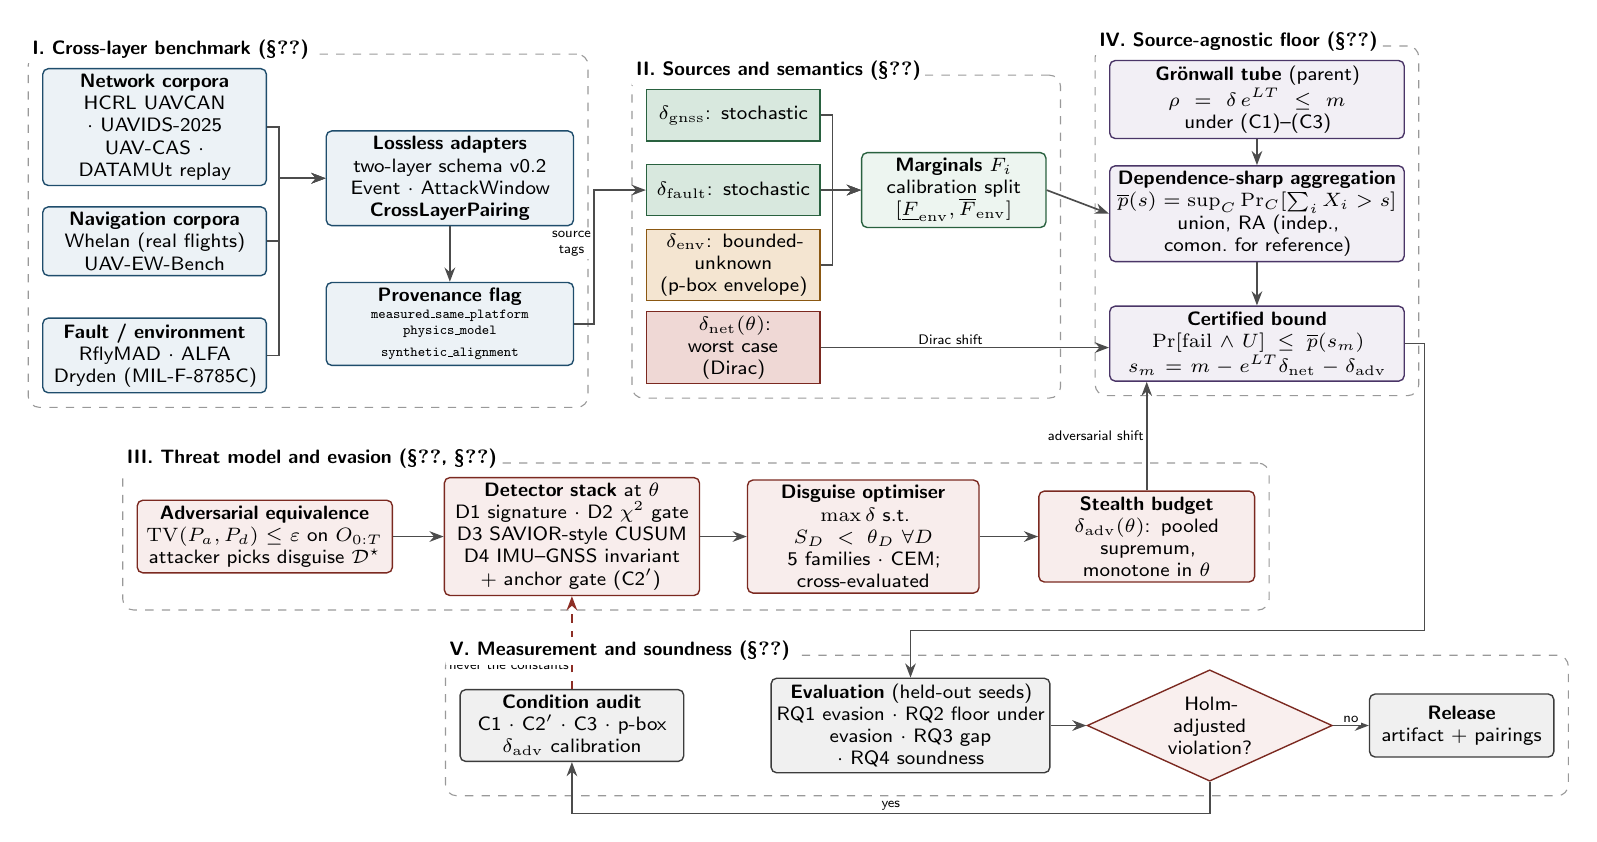
\begin{tikzpicture}[
  font=\sffamily\scriptsize,
  >={Stealth[length=1.8mm]},
  box/.style={draw=#1!70!black, fill=#1!8, rounded corners=2pt, align=center,
              minimum height=9mm, text width=#1W, inner sep=2pt, line width=0.5pt},
  b/.style 2 args={draw=#1!70!black, fill=#1!9, rounded corners=2pt, align=center,
              minimum height=8mm, text width=#2, inner sep=2pt, line width=0.5pt},
  d/.style={draw=#1!70!black, fill=#1!20, align=center, minimum height=6.5mm,
              text width=21mm, inner sep=1.5pt, line width=0.5pt},
  dia/.style={draw=cRed!70!black, fill=cRed!8, diamond, aspect=2.2, align=center,
              inner sep=0pt, text width=15mm, line width=0.5pt},
  phase/.style={draw=black!40, dashed, rounded corners=4pt, inner sep=5pt},
  ptitle/.style={font=\sffamily\bfseries\scriptsize, fill=white, inner sep=1.5pt, anchor=west},
  arr/.style={->, line width=0.6pt, draw=black!70},
  fb/.style={->, line width=0.6pt, draw=cRed!80!black, dashed},
  lab/.style={font=\sffamily\tiny, fill=white, inner sep=0.8pt, align=center},
]
% ======================= top track ======================================
% Phase I
\node[b={cBlue}{27mm}] (net) at (0, 0.2)  {\textbf{Network corpora}\\HCRL UAVCAN $\cdot$ UAVIDS-2025\\UAV-CAS $\cdot$ DATAMUt replay};
\node[b={cBlue}{27mm}] (nav) at (0,-1.25) {\textbf{Navigation corpora}\\Whelan (real flights)\\UAV-EW-Bench};
\node[b={cBlue}{27mm}] (flt) at (0,-2.7)  {\textbf{Fault / environment}\\RflyMAD $\cdot$ ALFA\\Dryden (MIL-F-8785C)};
\node[b={cBlue}{30mm}] (schema) at (3.75,-0.45) {\textbf{Lossless adapters}\\two-layer schema v0.2\\Event $\cdot$ AttackWindow\\\textbf{CrossLayerPairing}};
\node[b={cBlue}{30mm}] (prov) at (3.75,-2.3) {\textbf{Provenance flag}\\{\tiny\texttt{measured\_same\_platform}\\\texttt{physics\_model}\\\texttt{synthetic\_alignment}}};
\draw[arr] (net.east) -- ++(1.5mm,0) |- (schema.west);
\draw[arr] (nav.east) -- ++(1.5mm,0) |- (schema.west);
\draw[arr] (flt.east) -- ++(1.5mm,0) |- (schema.west);
\draw[arr] (schema) -- (prov);
% Phase II
\node[d=cGreen]  (dgnss)  at (7.35, 0.35) {$\dgnss$: stochastic};
\node[d=cGreen]  (dfault) at (7.35,-0.6)  {$\dfault$: stochastic};
\node[d=cOrange] (denv)   at (7.35,-1.55) {$\denv$: bounded-unknown\\(p-box envelope)};
\node[d=cRed]    (dnet)   at (7.35,-2.6)  {$\dnet(\theta)$: worst case\\(Dirac)};
\node[b={cGreen}{22mm}] (marg) at (10.15,-0.6) {\textbf{Marginals} $F_i$\\calibration split\\$[\underline F_{\mathrm{env}},\overline F_{\mathrm{env}}]$};
\draw[arr] (dgnss.east) -- ++(1.5mm,0) |- (marg.west);
\draw[arr] (dfault.east) -- (marg.west);
\draw[arr] (denv.east) -- ++(1.5mm,0) |- (marg.west);
\draw[arr] (prov.east) -- ++(2.5mm,0) |- node[lab, pos=0.3, left] {source\\tags} (dfault.west);
% Phase IV
\node[b={cPurple}{36mm}] (gron)  at (14.0, 0.55) {\textbf{Gr\"onwall tube} (parent)\\$\rho=\delta\,e^{LT}\le m$\\under (C1)--(C3)};
\node[b={cPurple}{36mm}] (agg)   at (14.0,-0.9) {\textbf{Dependence-sharp aggregation}\\$\overline p(s)=\sup_{C}\Pr_C[\sum_i X_i>s]$\\union, RA (indep., comon.\ for reference)};
\node[b={cPurple}{36mm}] (floor) at (14.0,-2.55) {\textbf{Certified bound}\\$\Pr[\mathrm{fail}\wedge U]\le\overline p(s_m)$\\$s_m=m-e^{LT}\dnet-\delta_{\mathrm{adv}}$};
\draw[arr] (marg.east) -- (agg.west);
\draw[arr] (gron) -- (agg);
\draw[arr] (agg) -- (floor);
\draw[arr] (dnet.east) -- node[lab, pos=0.45, above] {Dirac shift} (floor.west |- dnet.east);
% ======================= middle track (Phase III) ======================
\node[b={cRed}{31mm}] (threat) at (1.4,-5.0) {\textbf{Adversarial equivalence}\\$\mathrm{TV}(P_a,P_d)\le\varepsilon$ on $O_{0:T}$\\attacker picks disguise $\mathcal D^\star$};
\node[b={cRed}{31mm}] (dets)   at (5.3,-5.0) {\textbf{Detector stack} at $\theta$\\D1 signature $\cdot$ D2 $\chi^2$ gate\\D3 SAVIOR-style CUSUM\\D4 IMU--GNSS invariant\\+ anchor gate (C2$'$)};
\node[b={cRed}{28mm}] (opt)    at (9.0,-5.0) {\textbf{Disguise optimiser}\\$\max\delta$ s.t.\ $S_D<\theta_D\ \forall D$\\5 families $\cdot$ CEM;\\ cross-evaluated};
\node[b={cRed}{26mm}] (dadv)   at (12.6,-5.0) {\textbf{Stealth budget}\\$\delta_{\mathrm{adv}}(\theta)$: pooled\\supremum, monotone in $\theta$};
\draw[arr] (threat) -- (dets);
\draw[arr] (dets) -- (opt);
\draw[arr] (opt) -- (dadv);
\draw[arr] (dadv.north) -- node[lab, pos=0.5, left] {adversarial shift} (dadv.north |- floor.south);
% ======================= bottom track (Phase V) =========================
\node[b={cGray}{34mm}] (eval)  at (9.6,-7.4) {\textbf{Evaluation} (held-out seeds)\\RQ1 evasion $\cdot$ RQ2 floor under\\evasion $\cdot$ RQ3 gap $\cdot$ RQ4 soundness};
\node[dia] (sound) at (13.4,-7.4) {Holm-adjusted\\violation?};
\node[b={cGray}{27mm}] (audit) at (5.3,-7.4) {\textbf{Condition audit}\\C1 $\cdot$ C2$'$ $\cdot$ C3 $\cdot$ p-box\\$\delta_{\mathrm{adv}}$ calibration};
\node[b={cGray}{22mm}] (rel)   at (16.6,-7.4) {\textbf{Release}\\artifact + pairings};
\draw[arr] (floor.east) -- ++(2.5mm,0) |- ([yshift=6mm]eval.north) -- (eval.north);
\draw[arr] (eval) -- (sound);
\draw[arr] (sound.south) -- ++(0,-4mm) -| node[lab, pos=0.25, above] {yes} (audit.south);
\draw[arr] (sound.east) -- node[lab, above] {no} (rel.west);
\draw[fb] (audit.north) -- node[lab, left, pos=0.35] {revise the model,\\never the constants} (dets.south);
% ======================= phase frames ===================================
\begin{scope}[on background layer]
\node[phase, fit=(net)(flt)(schema)(prov)] (P1) {};
\node[phase, fit=(dgnss)(dnet)(marg)] (P2) {};
\node[phase, fit=(gron)(floor)] (P4) {};
\node[phase, fit=(threat)(dets)(opt)(dadv)] (P3) {};
\node[phase, fit=(eval)(sound)(audit)(rel)] (P5) {};
\end{scope}
\node[ptitle] at ([yshift=0.5mm]P1.north west) {I.\ Cross-layer benchmark (\S\ref{sec:benchmark})};
\node[ptitle] at ([yshift=0.5mm]P2.north west) {II.\ Sources and semantics (\S\ref{sec:budget})};
\node[ptitle] at ([yshift=0.5mm]P4.north west) {IV.\ Source-agnostic floor (\S\ref{sec:budget})};
\node[ptitle] at ([yshift=0.5mm]P3.north west) {III.\ Threat model and evasion (\S\ref{sec:threat}, \S\ref{sec:evasion})};
\node[ptitle] at ([yshift=0.5mm]P5.north west) {V.\ Measurement and soundness (\S\ref{sec:eval})};
\end{tikzpicture}}
\caption{Methodological framework. Phase~I unifies network, navigation, fault and
environment corpora under one schema whose unit of record is the cross-layer
pairing, each carrying a mandatory provenance flag. Phase~II assigns every
perturbation source its probabilistic semantics and estimates its marginal on a
calibration split. Phase~III formalises adversarial equivalence and searches,
for each detector stack and operating point~$\theta$, for the disguise that
maximises undetected deviation; the pooled supremum is the stealth budget
$\delta_{\mathrm{adv}}(\theta)$. Phase~IV aggregates the stochastic and
bounded-unknown terms with dependence-sharp bounds and shifts the result by the
deterministic terms, yielding a certified floor that does not depend on which
source produced the perturbation. Phase~V tests that floor on held-out attackers
and rollouts; a Holm-significant violation triggers an audit of the stated
conditions rather than a re-tuning of constants (dashed feedback).}
\label{fig:framework}
\end{figure*}

\subsection{Navigation loop and mission completion}
Let $x(t)\in\R^n$ be the navigation state of the aircraft and
$\dot x=F(x,u)$ its closed-loop dynamics under feedback $u$ computed from the
\emph{estimated} state $\hat x$. A mission $\omega$ of horizon $T$ follows a
nominal path $x^{\mathrm{nom}}$ inside a corridor of half-width (margin) $m$.
Writing $e(t)$ for the cross-track deviation of the true position from the
nominal path, the mission completes if and only if
\begin{equation}
\label{eq:complete}
\textstyle \sup_{t\in[0,T]}|e(t)|\le m .
\end{equation}
The mission-completion rate is
$\MCR=\Pr_{\omega\sim\mathcal M}[\eqref{eq:complete}]$ for a stated mission
distribution $\mathcal M$; it is a population quantity, not a statement about
any single flight~\cite{paperII}.

\paragraph{The parent chain.}
If $F$ is $L$-Lipschitz on the operating region (condition C1) and the
navigation input is perturbed by at most $\delta$, Gr\"onwall's
inequality~\cite{gronwall1919} bounds the deviation over a certification
horizon $T_c$ by the tube radius $\rho=\delta e^{LT_c}$. For the relay-delay
attacker, the companion paper~\cite{parentpaper} proved a residual-budget lemma:
an attacker below a detector threshold $\theta$ on $H$ malicious hops hides at
most $\Delta(\theta)\le H\min(\theta,s)$ of staleness, with the contact-window
slack $s$ measured at \nParentSlack\,s over \nParentHops{} relay hops. It also
calibrated the delay-to-position rate on real jamming and spoofing flights at
the supremum $\gamma=\nParentGamma$\,m/s. The network contribution to the
deviation is therefore at most
\begin{equation}
\label{eq:dnet}
e^{LT_c}\,\dnet(\theta),\qquad \dnet(\theta)=\gamma\,H\min(\theta,s),
\end{equation}
with the measured local Lipschitz constant $L=\nParentL$ and $T_c=1$\,s. At
the paper operating point ($\theta=0.25$\,s, $H=2$) this contributes
\nNetTubeQuarter\,m.

\subsection{Perturbation sources and their semantics}
Five sources perturb the navigation loop. They differ not only in magnitude
but in the \emph{kind of statement} that can be made about them:

\begin{center}\small
\begin{tabularx}{\columnwidth}{@{}l>{\raggedright\arraybackslash}X>{\raggedright\arraybackslash}X@{}}
\toprule
\textbf{Term} & \textbf{Origin} & \textbf{Semantics} \\
\midrule
$\dnet(\theta)$ & relay delay below $\theta$ & deterministic worst case \\
$\dadv(\theta)$ & disguised GNSS offset below the detector stack at $\theta$ & deterministic worst case (stealth budget) \\
$\dgnss$ & noise, Gauss--Markov drift, outages, jamming noise & stochastic, known marginal \\
$\dfault$ & inertial bias steps and drift, actuator loss of effectiveness & stochastic, known marginal \\
$\denv$ & turbulence within a declared intensity range & bounded-unknown (p-box) \\
\bottomrule
\end{tabularx}
\end{center}

\noindent
A deterministic term is a number that holds for every admissible behaviour. A
stochastic term has a cumulative distribution function (CDF) that we estimate
on a calibration split. A bounded-unknown term has a distribution known only to
lie between a lower and an upper CDF, a probability box~\cite{ferson2003}. For
wind, the box is spanned by the Dryden turbulence model of
MIL-F-8785C~\cite{milf8785c} between light and moderate intensity. What the
sources do \emph{not} come with is a joint distribution. Nature couples gusts and
outages in ways nobody has measured, and an attacker who induces jamming can
choose when GNSS degradation coincides with gusts.

\subsection{Problem statement}
Given (i)~the marginal laws of the stochastic sources, (ii)~an envelope for the
bounded-unknown source, (iii)~a detector stack operating at false-positive
rate (FPR) budget $\alpha$ with thresholds $\theta$, and (iv)~an attacker free
to choose both the shape of its interference and its coupling to the benign
sources, we seek:
\begin{description}[leftmargin=1.6em,style=sameline]
\item[P1] an upper bound on the probability that a mission fails
  \emph{and} its attack goes undetected, valid for every coupling of the benign
  sources and every attacker, i.e., a \emph{source-agnostic} bound;
\item[P2] a characterisation of how much tightness each aggregation rule
  sacrifices and where the slack comes from;
\item[P3] a measurement substrate that keeps the evidence behind every coupling
  explicit, and an evasion study that measures which disguise defeats which
  detector.
\end{description}
\noindent These define six research questions. RQ1: can an attacker mimic a
fault, a GNSS drift or a gust well enough to evade a detector while still
producing a large deviation, and which disguise does each detector miss? RQ2:
does the source-agnostic floor bound the outcome of missions whose attack went
undetected? RQ3: how loose are the union bound and the dependence-sharp bound in
practice, and is the looseness due to dependence or to time? RQ4: is the floor
sound at every held-out operating point under Holm-corrected tests, and does the
test detect unsoundness when a condition is deliberately broken? RQ5: does the
answer to RQ4 survive stronger attackers and a larger test, and if not, which
condition fails? RQ6: how much does the floor change when the simulated GNSS
marginal is replaced by measured jamming data?

\Cref{fig:framework} summarises the methodology through which the paper answers
these questions.

% =====================================================================
\section{Threat Model: Adversarial Equivalence}
\label{sec:threat}
% =====================================================================
\subsection{Capabilities, knowledge and goal}
The attacker can (a) delay relayed messages on up to $H$ hops of the mesh, as in
the companion paper, and (b) add an offset $d(t)$ to the GNSS position the
navigation filter receives. Capability (b) is realised in practice by
signal-level spoofing~\cite{humphreys2008,tippenhauer2011,kerns2014}; in this
paper it is exercised only through simulator interfaces. The attacker cannot
corrupt the inertial measurement unit (IMU), and it cannot corrupt a trusted
re-anchoring fix, such as a visual landmark or an authenticated position
broadcast, that arrives at least once every $T_a$ seconds (condition C2$'$, which
generalises the parent's re-anchoring condition from the network channel to the
GNSS channel). We return to IMU injection~\cite{son2015,trippel2017} in
\cref{sec:discussion}.

Following Kerckhoffs's principle, the attacker knows the detector designs and
their thresholds. It also observes the local wind, which a co-located attacker
can measure. It does not know the realisation of the benign noise. Its goal is to
maximise the vehicle's cross-track deviation while raising no alarm at any time
during the mission. Being detected late counts as being detected.

\subsection{Observational equivalence}
Let $O_{0:T}$ denote everything the defender observes: GNSS fixes, IMU samples,
commanded accelerations and anchor fixes. Write $P_a$ for the law of $O_{0:T}$
under attack $a$ (with the benign sources present), and $P_d$ for its law under a
benign disturbance $d$ drawn from a class $\Dclass$, such as inertial-bias drift,
GNSS multipath drift, or turbulence of a given intensity.

\begin{definition}[$\varepsilon$-observational equivalence]
\label{def:equiv}
Attack $a$ is $\varepsilon$-equivalent to the class $\Dclass$ if
$\inf_{d\in\Dclass}\TV(P_a,P_d)\le\varepsilon$, where
$\TV(P,Q)=\sup_A|P(A)-Q(A)|$ over measurable events $A$.
\end{definition}

\begin{lemma}[Detection advantage; Le Cam]
\label{lem:lecam}
For every detector $\psi:O_{0:T}\to\{0,1\}$ and every $d\in\Dclass$,
$\Pr_a[\psi=1]\le\Pr_d[\psi=1]+\TV(P_a,P_d)\le\Pr_d[\psi=1]+\sqrt{\KL(P_a\|P_d)/2}$.
\end{lemma}
\begin{proof}
The event $\{\psi=1\}$ is measurable, so $|P_a(\psi=1)-P_d(\psi=1)|\le\TV(P_a,P_d)$
by definition. The second inequality is Pinsker's~\cite{tsybakov2009}.
\end{proof}

\noindent
\Cref{lem:lecam} unifies three earlier notions. The ``hidden'' attacks of Hashemi
et al.\ raise alarms at the false-alarm rate~\cite{hashemi2018}; the
$\varepsilon$-stealthy attacks of Bai et al.\ bound the Kullback--Leibler (KL)
divergence~\cite{bai2017}; and the fault-mimicking attacks of Roy and Dey are the
noiseless case $\varepsilon=0$ in which $\Dclass$ is a fault class~\cite{roy2023}.
A detector with false-alarm rate $\alpha$ on $\Dclass$ thus catches an
$\varepsilon$-equivalent attack with probability at most $\alpha+\varepsilon$,
whatever its design.

\begin{definition}[Disguise-optimal attacker]
\label{def:disguise}
For a detector stack $\Psi_\theta=\{\psi_{D,\theta_D}\}_D$ and disguise families
$\{\Dclass_k\}$, each parameterised by $\phi\in\Phi_k$, the attacker solves
\begin{equation}
\label{eq:attacker}
\delta^\star_k(\theta)=\sup_{\phi\in\Phi_k}\ \E\big[\,\Delta_\phi\cdot
\mathbb 1\{\psi_{D,\theta_D}(O^\phi)=0\ \forall D\}\big],
\end{equation}
where $\Delta_\phi=\sup_t|e(t)|$ is the induced deviation. It then selects
$k^\star(\theta)=\arg\max_k\delta^\star_k(\theta)$. Dressing as the weather means
choosing $k^\star$ to be the class the stack tolerates most.
\end{definition}

\begin{proposition}[Detector-gated certificates and equivalence]
\label{prop:gated}
Let $\psi$ have false-alarm probability at most $\alpha$ under every
$d\in\Dclass$, and let $f_\Dclass$ be a floor valid under $\Dclass$. Let $a$ be
$\varepsilon$-equivalent to $\Dclass$ with $\alpha+\varepsilon<1$, and let
$q_a=\Pr_a[\text{fail}\mid\psi=0]$. Then
\[
\MCR_a\;\le\;1-q_a\,(1-\alpha-\varepsilon).
\]
Hence $f_\Dclass$ is violated by $a$ whenever
$q_a(1-\alpha-\varepsilon)>1-f_\Dclass$. A floor that is to remain valid against
every such attack must therefore bound the deviation the attack itself causes
on undetected missions; the detector's silence is no evidence of benignity.
\end{proposition}
\begin{proof}
By \cref{lem:lecam}, $\Pr_a[\psi=0]\ge\Pr_d[\psi=0]-\varepsilon\ge1-\alpha-\varepsilon$.
Then $1-\MCR_a\ge\Pr_a[\text{fail}\wedge\psi=0]=q_a\Pr_a[\psi=0]$.
\end{proof}

\noindent
The proposition is the formal content of ``the decisive attack is the one that
looks benign''. Without condition C2$'$, Khazraei et al.\ show that a GPS-only
attacker can make the undetected deviation grow without bound in an
incrementally exponentially stable closed loop~\cite{khazraei2024}, so $q_a$
approaches one for any fixed corridor. With C2$'$, the deviation an undetected attacker
can accumulate is limited by the anchor interval. The stealth budget
$\dadv(\theta)$ of \cref{sec:budget} is our estimate of that limit.

% =====================================================================
\section{The Unified Budget and the Source-Agnostic Floor}
\label{sec:budget}
% =====================================================================
\subsection{From sources to an additive budget}
For each benign source $i\in\{\mathrm{gnss},\mathrm{fault},\mathrm{env}\}$, let
$e_i(t)$ be the deviation the closed loop would exhibit under source $i$ alone,
and define its \emph{sup-deviation} $X_i=\sup_t|e_i(t)|$. Let $e_{\mathrm{adv}}$
be the deviation under the attack alone.

\begin{lemma}[Sub-additivity for additive inputs]
\label{lem:subadd}
Fix the time-varying parameters of a mission (GNSS outage schedule, actuator
effectiveness, anchor schedule). If the closed loop is then linear in its
additive inputs (wind force, sensor noise and bias, attack offset), the
deviation decomposes as $e=e_{\mathrm{ben}}+e_{\mathrm{adv}}$, and
$\sup_t|e(t)|\le\sup_t|e_{\mathrm{ben}}(t)|+\sup_t|e_{\mathrm{adv}}(t)|$.
\end{lemma}
\begin{proof}
Superposition for a linear time-varying system, then the triangle inequality.
\end{proof}

\noindent
Two remarks bound the lemma's reach. First, actuator saturation is not linear,
so the lemma holds only inside the region where (C1) holds; the parent paper
excludes saturation from that region for the same reason~\cite{parentpaper}.
Second, outages and loss of effectiveness are \emph{parametric} sources: they
change the system rather than add an input. The further decomposition of
$e_{\mathrm{ben}}$ into per-source suprema,
$\sup_t|e_{\mathrm{ben}}|\le\sum_iX_i$, is therefore an assumption, which we
state as condition (C5) and test mission by mission in \cref{sec:eval}.

\subsection{Dependence-sharp aggregation}
Because the $X_i$ share no known joint law, we bound the tail of their sum over
\emph{all} couplings consistent with the marginals. For non-negative $X_1,\dots,X_d$
with survival functions $S_i(t)=\Pr[X_i>t]$, define the worst-case and standard bounds
\begin{align}
\pbar(s)&=\sup_{C}\Pr_C\Big[\textstyle\sum_{i}X_i>s\Big],\\
p_U(s)&=\min\Big\{1,\ \inf_{s_1+\dots+s_d=s}\textstyle\sum_iS_i(s_i)\Big\},
\end{align}
where the supremum runs over all copulas $C$.

\begin{proposition}[Tightness of the union bound]
\label{prop:union}
(a)~$\pbar(s)\le p_U(s)$ for all $s$.
(b)~For $d=2$, $\pbar=p_U$ at every continuity point: the union bound is
sharp~\cite{makarov1981,ruschendorf1982,frank1987}.
(c)~For $d\ge3$ the inequality can be strict; the Rearrangement Algorithm (RA)
approximates $\pbar$, with excellent empirical accuracy but no general
convergence proof~\cite{puccetti2012,embrechts2013var}.
(d)~Against a known benign coupling $C_0$, the ratio
$p_U(s)/\Pr_{C_0}[\sum X_i>s]$ never exceeds $d$ under comonotonicity (take
$s_i=F_i^{-1}(u)$) and equals $d$ for identically distributed comonotone sources
whenever the equal split is optimal. Under independence it is unbounded: for two independent
$\mathrm{Exp}(1)$ sources, $p_U(s)\approx2e^{-s/2}$ while the truth is
$(1+s)e^{-s}$.
(e)~A deterministic term $X_j\equiv c$ has a single coupling with any other
variable, so it shifts $s$ by $c$ and contributes no dependence gap.
\end{proposition}
\begin{proof}
(a) For any split, $\{\sum X_i>s\}\subseteq\bigcup_i\{X_i>s_i\}$. (b) is
Makarov's theorem~\cite{makarov1981}, proved independently by
R\"uschendorf~\cite{ruschendorf1982}; Frank et al.\ give the
attaining coupling~\cite{frank1987}. (c) Embrechts et al.\ give examples of
strict inequality and the RA~\cite{embrechts2013var}. (d) is direct
computation; for independent exponentials, $p_U$ is attained at the equal split
and the ratio $2e^{s/2}/(1+s)$ diverges. (e) The Fr\'echet class of a Dirac
marginal is a singleton.
\end{proof}

\noindent
\paragraph{Who chooses the coupling?}
The adversarial offset enters as a deterministic term, so by (e) it has no
coupling to choose. The dependence-sharp bound is needed for two other
reasons. First, nature's coupling of gusts, outages and faults has never been
measured. Second, an attacker who controls a \emph{stochastic} source, for
example by jamming to induce the outages and noise of $\dgnss$, chooses when
that source fires relative to the others, and hence its coupling, provided the
induced episodes leave the marginal of $X_{\mathrm{gnss}}$ within its
calibration (C3). Our proposal
had hypothesised that a joint treatment recovers the union bound's slack
precisely when the sources are comonotone. \Cref{prop:union} corrects this.
When the coupling is unknown or adversarial, the union bound is already the
right quantity for two sources and nearly right for three. The slack exists only
relative to a coupling that is \emph{known} to be benign.

\subsection{The floor}
\begin{theorem}[Source-agnostic, dependence-sharp bound]
\label{thm:floor}
Assume (C1)~a Lipschitz, unsaturated closed loop; (C2$'$)~a trusted re-anchoring
fix at least every $T_a$ seconds, including at the end of the mission; (C3)~transfer
of the calibrated interface quantities ($\gamma$, the marginals of $X_i$, and
the stealth budget $\dadv$) to the deployment; (C4)~an environmental marginal in
the declared envelope, with CDFs
$\underline F_{\mathrm{env}}\le F_{\mathrm{env}}\le\overline F_{\mathrm{env}}$; and
(C5)~sub-additivity across benign sources. Let $U$ be the event that the stack
$\Psi_\theta$ raises no alarm. Then, for every coupling of the benign sources and
every attack,
\begin{align}
\Pr[\text{fail}\wedge U]\ &\le\ \pbar\big(s_m\big),\qquad
s_m=m-e^{LT_c}\dnet(\theta)-\dadv(\theta),\label{eq:floor}
\end{align}
with $\pbar$ evaluated at the stochastically largest environmental marginal,
whose CDF is $\underline F_{\mathrm{env}}$. Consequently
$\Pr[\text{complete}\mid U]\ge1-\pbar(s_m)/\Pr[U]$, and in the population of
all missions $\Pr[\text{fail}\wedge U]\le1-f(m)$ with $f(m)=1-\pbar(s_m)$.
\end{theorem}
\begin{proof}
On $U$, (C3) gives $\sup_t|e_{\mathrm{adv}}|\le\dadv$, so by \cref{lem:subadd} and
(C5), failure on $U$ implies $\sum_iX_i>s_m$. Hence
$\Pr[\text{fail}\wedge U]\le\Pr[\sum_iX_i>s_m]\le\pbar(s_m)$, which needs no
conditioning on $U$. The tail of a sum is non-decreasing under first-order
stochastic dominance of any summand, for every coupling and hence for the
supremum, so the stochastically largest member of the p-box is the worst. The
conditional form follows by dividing by $\Pr[U]$.
\end{proof}

\begin{remark}
The theorem is conditional in exactly the sense of the parent
guarantee~\cite{parentpaper}: its first and last links are proved, and its
interface quantities are measured. We therefore test (C3)--(C5) empirically
in \cref{sec:eval} instead of asserting them. Bounding the \emph{joint} event
$\{\text{fail}\wedge U\}$, rather than the completion rate conditional on
silence, is what lets the bound use unconditional benign marginals: conditioning
on silence would select benign realisations and change their law.
\end{remark}

\subsection{Computing the floor}
The marginals are estimated on a calibration split (seed block 1xxx) from
\nCalMissions{} missions per source. $p_U$ is minimised over a grid of splits.
$\pbar$ is approximated by the RA with $N=1{,}000$ quantile levels, using both the
upper and the lower discretisation, keeping the larger value, and bisecting on
the confidence level~\cite{embrechts2013var,hofert2020}. $p_U$ is a proven upper
bound on $\pbar$; the RA value, with the conservative discretisation, is a
numerical approximation of $\pbar$ that is not proven in general. We report
$\min(\mathrm{RA},p_U)$ as our estimate of $\pbar$, which also removes the RA's
$1/N$ resolution floor in the far tail, and we give $p_U$ alongside wherever a
bound must be strictly certified. For reference only, we
also report the tail under independence (Monte Carlo) and under comonotonicity
(quantile sum). Neither is a certificate.

% =====================================================================
\section{The Cross-Layer Benchmark}
\label{sec:benchmark}
% =====================================================================
A guarantee that spans layers needs data objects that record the coupling
between them, and no public corpus provides such objects. The benchmark extends
the parent's two-layer schema~\cite{parentpaper}. Its three record kinds are an
\emph{Event} (an atomic observation), an \emph{AttackWindow} (a labelled
interval) and a \emph{CrossLayerPairing}, which joins a network or environmental
window to the navigation window it induces. A pairing carries the detector
operating point, the residual budget, the induced perturbation and the mission
outcome. Version~0.2 adds a \code{perturbation\_source} field taking values
\code{net}, \code{gnss}, \code{fault}, \code{env} or \code{adv}, so that fault and
environment pairings share the attack pairings' representation.

\paragraph{Provenance is mandatory.}
Every pairing carries one of three flags:
\code{measured\_same\_platform} (both windows observed on one airframe),
\code{physics\_model} (coupled through a stated physical relation) or
\code{synthetic\_alignment} (aligned in simulation). Readers can therefore
filter by strength of evidence rather than trust an unaudited join. The flag
keeps the most important qualification in plain view. Of the six corpora, only
the UAV Attack Dataset~\cite{whelan2020dataset,whelan2020novelty} observes a
network or radio event and the flight it degrades on the same platform, and its
release carries no machine-readable attack intervals. The number of released
\code{measured\_same\_platform} pairings is therefore zero, and every record of the
benchmark says so.

\paragraph{Contents.}
Lossless adapters ingest the HCRL UAVCAN bus corpus~\cite{kim2022uavcan},
UAVIDS-2025~\cite{zeng2025uavids}, UAV-CAS~\cite{mishra2026uavcas}, a replay of
the DATAMUt time-delay detector~\cite{soltani2026datamut}, the UAV Attack
Dataset, and the physics-informed UAV-EW-Bench~\cite{uavewbench2026}. Together
these give \nEventsTotal{} events, of which \nEventsReal{} were captured on real
hardware. Each adapter is verified by a hash round-trip, so that no source
column is discarded. Fault and environment sources enter through the
RflyMAD~\cite{le2025rflymad} and ALFA~\cite{keipour2021alfa} fault taxonomies
and the Dryden model~\cite{milf8785c}. The benchmark ships a detector-operating-curve
harness that sweeps $\theta$, the dependence-bound library (union, RA,
independence, comonotone), the disguise-evasion harness of \cref{sec:evasion},
and datasheets~\cite{gebru2021} that map each pitfall of Arp et
al.~\cite{arp2022dos} to its mitigation. Third-party data is fetched from its
origin under its own licence. We release adapters and unified labels, never
redistributed corpora. In this paper the benchmark supplies the interface
constants of the network term ($\gamma$, $s$, $L$; the event totals come from the
parent's provenance ledger). The evasion study itself runs in simulation, and
its records enter the benchmark with the provenance flag \code{synthetic\_alignment}.

% =====================================================================
\section{Evasion Study Design}
\label{sec:evasion}
% =====================================================================
\subsection{Closed loop and perturbation models}
The pilot models the lateral (cross-track) channel of a small multirotor
cruising at $V=8$\,m/s through a 60\,s mission segment. The airframe is a
drag-damped double integrator, $\ddot p=u+c_d(w-\dot p)$ with $c_d=0.35$\,s$^{-1}$.
It is driven by a proportional--derivative (PD) controller acting on the KF
estimate and saturated at 4\,m/s$^2$. The KF has states (position, velocity,
accelerometer bias), propagates with the 20\,Hz accelerometer, and corrects
with 10\,Hz GNSS fixes and the anchor fix every $T_a=5$\,s.

\emph{Environment.} The lateral wind $w$ follows the Dryden spectrum of
MIL-F-8785C at 100\,ft altitude. With $W_{20}$ the wind speed at 20\,ft, it has
$\sigma_v=0.1W_{20}/(0.177+0.000823h)^{0.4}$ and scale length
$L_v=h/(0.177+0.000823h)^{1.2}$. The declared envelope is
$W_{20}\in[15,30]$\,kt (light to moderate); severe turbulence (45--60\,kt) lies
outside it and serves as a negative control. Because the accelerometer measures
the aerodynamic force, wind is consistent between the IMU and GNSS, as it is on
a real airframe to first order.

\emph{Faults.} Faults are drawn independently per mission: an accelerometer bias
step (probability 0.3, $\sigma=0.1$\,m/s$^2$); bias drift (0.2, with the random
walk inflated tenfold); and actuator loss of effectiveness (LoE) of 10--30\%
(0.2).

\emph{GNSS.} Noise has a white component ($\sigma=0.5$\,m) and a first-order
Gauss--Markov drift ($\sigma=0.8$\,m, $\tau=60$\,s). Outages are
exponential with mean 5\,s (probability 0.3), and jamming-noise episodes
triple $\sigma$ for 10\,s (probability 0.2).

\subsection{Detectors}
All four detectors observe only $O_{0:T}$. Each reduces a mission to one
statistic $S_D$ and alarms when $S_D>\theta_D$:
\begin{description}[leftmargin=1em,style=nextline]
\item[D1, signature monitor.] $S_1=\max_k|z_k-z_{k-1}|$, the largest jump between
  consecutive fixes. It stands in for rule-based IDSs tuned to malicious
  signatures such as jumps and discontinuities.
\item[D2, $\chi^2$ innovation gate.] This is loosely modelled on innovation
  gating in PX4-class filters: it alarms when the normalised innovation squared
  (NIS) $\nu_k^2/S_k$ exceeds $\theta_2$ on three consecutive fixes. (PX4's EKF2
  rejects individual measurements rather than alarming.)
\item[D3, SAVIOR-style CUSUM.] A model-based observer driven by the commanded
  acceleration with a no-wind model accumulates a cumulative-sum (CUSUM)
  statistic $g_k=\max(0,g_{k-1}+r_k^2-(1+\kappa))$ on its GNSS
  residual~\cite{quinonez2020savior}.
\item[D4, IMU--GNSS invariant.] A quadratic is fitted over 4\,s to the residual
  between the GNSS position and the doubly integrated accelerometer; the
  detector alarms when the curvature, an acceleration discrepancy, exceeds
  $\theta_4$ on five consecutive fixes. It is the cross-sensor analogue of the
  control invariants of Choi et al.~\cite{choi2018}.
\end{description}
Whenever C2$'$ holds, an anchor gate on the anchor fix's NIS (calibrated FPR
1\%) is part of every stack. Thresholds are set on \nCalMissions{} benign
missions so that each detector has the stated per-mission FPR; the combined
stack \textsc{All} splits the budget equally among its four members.

\subsection{Disguise families and the attacker}
The offset $d(t)$, applied from an onset time $t_0$, belongs to one of five
families:
\begin{itemize}
\item \emph{step}: $d=A$ (the naive spoofer);
\item \emph{ramp}: $d=\min\{r(t-t_0),A\}$ (the ``boiling frog'');
\item \emph{fault mimic}: $\ddot d=\beta_0+\beta(t)$, with $\beta$ a random walk,
  capped at $|d|\le A$. It imitates accelerometer-bias drift, which the filter's
  bias state absorbs;
\item \emph{GNSS mimic}: $d=A|g(t)|+c(t-t_0)$, with $g$ a unit Gauss--Markov
  process of attacker-chosen correlation time, imitating multipath or
  ionospheric drift;
\item \emph{weather mimic}: $d=A\,w(t-\ell)/\sigma_{\mathrm{mod}}+b\min\{(t-t_0)/10,1\}$,
  where $\sigma_{\mathrm{mod}}$ is the moderate-turbulence $\sigma_v$. The offset
  follows the true gust with a lag $\ell$.
\end{itemize}
The attacker solves~\eqref{eq:attacker} with the cross-entropy method
(CEM)~\cite{rubinstein2004cem}: 12 candidates per generation, 4 elites,
\nCemGens{} generations and \nCemK{} missions per candidate. Each
(stack $\times$ family $\times$ operating point) combination gets its own
optimiser seed in block 2xxx; stronger optimisers (CMA-ES~\cite{hansen2016cma},
Bayesian optimisation) are runbook item R1. Because a local optimiser can fail
to find an evading parameterisation that exists, we do not read detector
strength off the optimiser's own target. Instead, we \emph{cross-evaluate} every
optimised attacker against every stack.

\subsection{Metrics and statistical protocol}
For each optimised attacker, evaluated on fresh missions (block 4xxx), we report:
\begin{itemize}
\item the \emph{evasion rate} (no alarm during the whole mission);
\item the attack's own contribution $\sup_t|e_{\mathrm{adv}}|$ on evading
  missions, computed on the same realisation with the additive benign inputs set
  to zero but the parametric ones (outages, LoE) kept, as in \cref{lem:subadd};
\item the Kolmogorov--Smirnov (KS) distance between each detector's statistic
  under attack and under benign conditions, a finite-sample estimate of the TV
  distance of \cref{lem:lecam} restricted to threshold tests.
\end{itemize}
In the cross-evaluated disguise matrix, a cell's contribution is the maximum
over attackers that evade in at least 5\% (and at least 10) of missions; we
report the unfiltered maxima separately. The stealth budget $\dadv(\theta)$ is
the supremum of the attack-only deviation over \emph{all} evading missions, with
no such filter. It is pooled over all \nPooledAttackers{} optimised
attackers on calibration missions (block 1xxx). Every attacker uses the same
missions at every operating point, and an attack that is stealthy against
stricter thresholds is also stealthy against looser ones, so the pooled
supremum is monotone in the operating point by construction.

For soundness, we re-optimise an independent attacker with fresh seeds (block
3xxx) for every family and FPR, against the full stack. We evaluate it on $n=\nEvalMissions$
fresh missions per operating point, crossing family, FPR, wind (light, moderate,
envelope), margin $m$ and $\theta_{\mathrm{net}}$. The theorem's event is
$\{\text{fail}\wedge U\}$, so we count its occurrences $k$ and compute the
one-sided binomial $p$-value of $H_0{:}\ \Pr[\text{fail}\wedge U]\le\pbar(s_m)$.
The $p$-values are adjusted across all operating points by Holm's
procedure~\cite{holm1979}, and a violation is a Holm-adjusted $p<0.05$. We
also report the MCR conditional on $U$, with Clopper--Pearson
intervals~\cite{clopper1934}.

% =====================================================================
\section{Evaluation}
\label{sec:eval}
% =====================================================================
% ------------------------------------------------------------- Results
% =====================================================================
% Results figures (pgfplots). Data: figdata/*.dat from make_numbers.py
% =====================================================================
\pgfplotsset{
  p4/.style={width=\columnwidth, height=4.6cm, grid=major, grid style={black!12},
    tick label style={font=\scriptsize}, label style={font=\footnotesize},
    legend style={font=\scriptsize, draw=none, fill=white, fill opacity=0.85, text opacity=1},
    every axis plot/.append style={line width=0.9pt}},
}

% ---------------- Fig: detector operating curves ------------------------
\newcommand{\figROC}{%
\begin{figure}[t]
\centering
\begin{tikzpicture}
\begin{axis}[p4, width=0.56\columnwidth, height=4.3cm, xmin=0, xmax=0.3, ymin=0, ymax=1.02,
  xlabel={FPR}, ylabel={TPR}, title={\scriptsize step offset, 5\,m},
  legend to name=rocleg, legend columns=4]
\addplot[cBlue] table[x=fpr,y=tpr]{figdata/roc_step_D1.dat}; \addlegendentry{D1 signature}
\addplot[cOrange, dashed] table[x=fpr,y=tpr]{figdata/roc_step_D2.dat}; \addlegendentry{D2 $\chi^2$}
\addplot[cGreen, dotted] table[x=fpr,y=tpr]{figdata/roc_step_D3.dat}; \addlegendentry{D3 SAVIOR-style}
\addplot[cRed, dashdotted] table[x=fpr,y=tpr]{figdata/roc_step_D4.dat}; \addlegendentry{D4 invariant}
\draw[black!50, densely dashed] (axis cs:0.05,0) -- (axis cs:0.05,1.02);
\end{axis}
\end{tikzpicture}%
\hfill
\begin{tikzpicture}
\begin{axis}[p4, width=0.56\columnwidth, height=4.3cm, xmin=0, xmax=0.3, ymin=0, ymax=1.02,
  xlabel={FPR}, yticklabels={}, title={\scriptsize ramp, 0.5\,m/s}]
\addplot[cBlue] table[x=fpr,y=tpr]{figdata/roc_ramp_D1.dat};
\addplot[cOrange, dashed] table[x=fpr,y=tpr]{figdata/roc_ramp_D2.dat};
\addplot[cGreen, dotted] table[x=fpr,y=tpr]{figdata/roc_ramp_D3.dat};
\addplot[cRed, dashdotted] table[x=fpr,y=tpr]{figdata/roc_ramp_D4.dat};
\draw[black!50, densely dashed] (axis cs:0.05,0) -- (axis cs:0.05,1.02);
\end{axis}
\end{tikzpicture}\\[-1pt]
\pgfplotslegendfromname{rocleg}
\caption{Detector operating curves against two \emph{naive} offsets, with
thresholds swept over \nCalMissions{} benign missions (dashed line: the 5\%
operating point). Only D2 and D4 separate a naive 5\,m step, and only D2
separates the ramp.}
\label{fig:roc}
\end{figure}}

% ---------------- Fig: anchor-interval sweep ----------------------------
\newcommand{\figAnchor}{%
\begin{figure}[t]
\centering
\begin{tikzpicture}
\begin{loglogaxis}[p4, height=4.4cm, xmin=4, xmax=25, ymin=1, ymax=400,  xtick={5,10,20}, xticklabels={5,10,20},
  xlabel={re-anchoring interval $T_a$ (s)}, ylabel={max.\ undetected contribution (m)},
  legend pos=north west, legend cell align=left]
\addplot[cRed, mark=square*, mark size=1.6pt, line width=1.2pt] table[x=Ta,y=maxall]{figdata/anchor_sweep_open.dat}; \addlegendentry{final interval unchecked}
\addplot[cBlue, mark=*, mark size=1.6pt, line width=1.2pt] table[x=Ta,y=maxall]{figdata/anchor_sweep.dat}; \addlegendentry{every interval closed (C2$'$)}

\end{loglogaxis}
\end{tikzpicture}
\caption{Stealth budget against the full stack (5\% FPR) versus the
re-anchoring interval, pooled over 30 attackers (15 tuned per $T_a$ and the 15
optimised against the full stack) and maximised over the five disguise
families, on the same missions at every $T_a$. With every interval closed, the
largest undetected contribution grows from \nAnchorMaxFive{} to
\nAnchorMaxTwenty\,m (\nAnchorMultTwenty$\times$). With the final segment
before mission end unchecked, it grows \nOpenMultTwenty$\times$ to
\nOpenMaxTwenty\,m.}
\label{fig:anchor}
\end{figure}}

% ---------------- Fig: dependence gap -----------------------------------
\newcommand{\figGap}{%
\begin{figure}[t]
\centering
\begin{tikzpicture}
\begin{semilogyaxis}[p4, height=4.8cm, xmin=2.5, xmax=8.5, ymin=1e-4, ymax=1.2,
  xlabel={budget available to benign sources $s$ (m)}, ylabel={$\Pr[\sum_i X_i>s]$},
  legend style={at={(0.5,-0.28)}, anchor=north, legend columns=2}]
\addplot[cPurple, line width=1.2pt] table[x=s,y=union]{figdata/gap.dat}; \addlegendentry{union bound}
\addplot[cPurple, dashed, line width=1.2pt] table[x=s,y=ra]{figdata/gap.dat}; \addlegendentry{RA (worst coupling)}
\addplot[cBlue, dashdotted] table[x=s,y=indep]{figdata/gap.dat}; \addlegendentry{indep., upper envelope}
\addplot[cGreen, densely dotted, line width=1.1pt] table[x=s,y=indepmix]{figdata/gap.dat}; \addlegendentry{indep., matched wind}
\addplot[cOrange, mark=x, mark size=1.6pt, only marks] table[x=s,y=sumsame]{figdata/gap.dat}; \addlegendentry{sum of suprema, same mission}
\addplot[cGray, mark=*, mark size=1pt, only marks] table[x=s,y=joint]{figdata/gap.dat}; \addlegendentry{joint simulation}
\end{semilogyaxis}
\end{tikzpicture}
\caption{Where the looseness lives (tail of the benign budget). Union and RA
nearly coincide. The steps down from RA are: to independent sums at the upper
wind envelope (dependence gap); to independent sums at the wind actually
flown (envelope gap); to the sum of per-source suprema on the same missions,
which confirms that the simulated sources are independent; and to the joint
simulation (temporal gap: sources seldom peak at the same instant).}
\label{fig:gap}
\end{figure}}

% ---------------- Fig: floor vs MCR --------------------------------------
\newcommand{\figFloor}{%
\begin{figure}[t]
\centering
\begin{tikzpicture}
\begin{axis}[p4, height=4.6cm, xmin=4, xmax=25, ymin=0, ymax=1.03,
  xlabel={corridor margin $m$ (m)}, ylabel={$1-\Pr[\mathrm{fail}\wedge U]$},
  legend style={at={(0.5,-0.28)}, anchor=north, legend columns=2}]
\addplot[cPurple, line width=1.3pt] table[x=m,y=ra]{figdata/floor_curve.dat}; \addlegendentry{$1-\pbar$, RA, $\theta_{\mathrm{net}}=0$}
\addplot[cPurple, dashed] table[x=m,y=ranet]{figdata/floor_curve.dat}; \addlegendentry{$1-\pbar$, RA, $\theta_{\mathrm{net}}=0.25$\,s}
\addplot[cBlue, dashdotted] table[x=m,y=indep]{figdata/floor_curve.dat}; \addlegendentry{independence (not certified)}
\addplot[cRed, mark=*, mark size=2pt, only marks] table[x=m,y=obs]{figdata/floor_points.dat}; \addlegendentry{measured $1-\Pr[\mathrm{fail}\wedge U]$}
\end{axis}
\end{tikzpicture}
\caption{Certified bound versus measurement at 5\% FPR. The measured
points are the worst case over five held-out attackers and three wind
conditions. The bound stays below every measurement. Including the network
term shifts it right by $e^{LT_c}\dnet=\nNetTubeQuarter$\,m.}
\label{fig:floor}
\end{figure}}

The pilot comprises \nMissionsTotal{} simulated missions and ran in
\nWallMin{} minutes on two CPU cores. Every number below is generated from the
released result files.

\subsection{Calibration: who sets the thresholds?}
At the 5\% operating point, the per-detector FPR stays between \nFprModMin{}
and \nFprModMax{} under moderate wind, and the anchor gate alone contributes
\nFprAnchor. One finding shapes everything that follows: \emph{wind and faults
alone trip no detector} (FPR \nFprWindFaultMax{} for every detector when either
is the only benign source), whereas GNSS error alone produces up to
\nFprGnssOnlyMax{}. The thresholds are therefore set by the tails of the GNSS
error, and the tolerance they grant is the space an attacker exploits. Severe
turbulence, outside the declared envelope, raises the FPR of the SAVIOR-style
detector D3, which models no wind, to \nFprSevereDThree{}; the others stay at or
below \nFprSevereOtherMax{}.

\Cref{fig:roc} shows the operating curves against naive offsets. At 5\% FPR the
$\chi^2$ gate detects a 5\,m step in \nTprStepDTwo{} of missions and the
invariant D4 in \nTprStepDFour{}, but the signature monitor and D3 detect it in
only \nTprStepDOne{} and \nTprStepDThree{}, which is close to chance. A 0.5\,m/s
ramp is caught by D2 (\nTprRampDTwo{}) and essentially by no other detector
($\le$\nTprRampDThree{}).

\figROC

\subsection{RQ1: evasion is universal; the damage is not}
\paragraph{Cross-evaluation.}
We evaluated each of the \nPooledAttackers{} optimised attackers against every
stack. In \nOwnOptFail{} of \nCells{} (stack, family) cells, the CEM run that
targeted that stack found no parameterisation evading in at least 5\% of
missions, although an attacker optimised for a different stack does. Reading detector strength off the
optimiser's own target would therefore have been wrong, so
\cref{tab:disguise} reports the best attacker of each family, wherever it was
optimised.

\paragraph{With the anchor gate, the anchor sets the budget.}
With condition C2$'$ in force and its gate armed (\cref{tab:disguise}, top),
every one of the five families evades every detector, and the full stack, in
at least \nCrossEvMin{} of missions; for reference, benign missions raise no
alarm in about \nBenignNoAlarm{} under the full stack. Each family has
parameterisations that offset GNSS by about 1--2\,m, and every detector must
tolerate offsets of that size to keep its FPR at 5\%. Among attackers that evade
in at least 5\% of missions, the largest undetected contribution lies between
\nDevSingleMin{} and \nDevSingleMax\,m \emph{whichever detector is deployed}.
Rarer evasions go further: up to \nGatedUnfMax\,m against \nGatedUnfStacks{}
(\nGatedUnfFam). The pooled supremum against the full stack is \nAnchorMaxFive\,m
(\cref{fig:anchor}), and the stealth budget is $\dadv=\nDadvFive$\,m. Within that
range the trusted fix, not the detector design, decides how far an undetected
attacker gets. The median KS distance between a detector's statistic under an
evading attack and under benign conditions is \nKsStealthyMed{}, against
\nKsCaughtMed{} for detected ones. This is the empirical face of
\cref{lem:lecam}: an attack that evades is, to the detector, almost
indistinguishable from the benign population.

\paragraph{Without the gate, each detector admits a different disguise.}
The bottom of \cref{tab:disguise} repeats the cross-evaluation with the anchor
still fused into the filter but its alarm removed, isolating what the detectors
themselves discriminate. Evasion stays at or above \nNgEvMin{}, but the
undetected contribution now depends sharply on the pairing of disguise and
detector.
\begin{itemize}
\item The fault mimic drives \nNgDOneFaultMimic{}\,m past D1, D3 and D4. Its slow,
  bias-shaped curvature has no jumps for D1, matches the bias drift that D4
  tolerates by design, and looks like an unmodelled disturbance to D3.
\item The GNSS mimic and the weather mimic exploit the two detectors that do
  not cross-check the IMU, D1 and D3 (up to \nNgDOneGnssMimic{} and
  \nNgDOneWeatherMimic\,m). Among frequently evading attackers, D4 caps them at
  \nNgDFourWeatherMimic\,m or below, because their acceleration content
  contradicts the accelerometer; a rare GNSS-mimic evasion still reached
  \nNgDFourGnssUnf\,m.
\item Rare step offsets that happen to land in a benign noise trough evade D1,
  D3 and D4 in about 3\% of missions and reach \nNgStepUnfMax\,m.
\item Only the $\chi^2$ gate D2, whose filter models the accelerometer bias,
  caps every family, at \nNgCapDTwo\,m (fault mimic), including rare evasions
  (\nNgDTwoUnfMax\,m); the full stack, which contains D2, is capped at
  \nNgCapALL\,m.
\end{itemize}
This is the pattern adversarial equivalence predicts. The disguise that wins
is the one the detector models as benign: bias drift for an invariant that
tolerates bias, and drift or wind-shaped motion for detectors without an
inertial cross-check.

\begin{table}[t]
\centering\footnotesize
\setlength{\tabcolsep}{3pt}
\caption{Disguise matrix at 5\% FPR, cross-evaluated over all
\nPooledAttackers{} optimised attackers on \nEvalMissions{} held-out missions
per attacker. \emph{Top:} anchor gate armed; best evasion rate (\%) / largest
undetected attack contribution (m). \emph{Bottom:} anchor fused but its gate
removed; largest undetected contribution (m). Contributions are taken over
attackers that evade in at least 5\% (and at least 10) of missions; rarer
evasions are reported in the text. Benign missions raise no alarm in about
\nBenignNoAlarm{}. Darker cells are evaded more often (top) or admit more
deviation (bottom).}
\label{tab:disguise}
\begin{tabular}{@{}lccccc@{}}
\toprule
& \textbf{step} & \textbf{ramp} & \textbf{fault} & \textbf{GNSS} & \textbf{weather} \\
& & & \textbf{mimic} & \textbf{mimic} & \textbf{mimic} \\
\midrule
\multicolumn{6}{@{}l}{\emph{anchor gate armed (C2$'$)}}\\
\tabinput{tab_disguise_body.tex}
\midrule
\multicolumn{6}{@{}l}{\emph{anchor fused, gate removed}}\\
\tabinput{tab_disguise_nogate_body.tex}
\bottomrule
\end{tabular}
\end{table}

\paragraph{The terminal window.}
\Cref{fig:anchor} sweeps the re-anchoring interval against the full stack,
pooling all attackers on common missions. With every interval closed, the
largest undetected contribution grows from \nAnchorMaxFive\,m at $T_a=5$\,s to
\nAnchorMaxTwenty\,m at 20\,s (\nAnchorMultTwenty$\times$). The attacker must
return near zero before each trusted fix, so the budget is set by how far it can
travel and come back within one interval. When the segment before mission end
is left unchecked, no return leg is needed, and the contribution reaches
\nOpenMaxTwenty\,m, \nOpenRatioTwenty$\times$ the closed value. The terminal
window is where an equivalence attacker spends its budget.

\figAnchor

\subsection{RQ3: where the looseness lives}
\Cref{fig:gap} decomposes the tail of the benign budget; the ratios below are
at $s=\nGapS$\,m, and their ordering changes in the far tail, where few joint
exceedances remain.
\begin{enumerate}
\item For two sources, the union and RA bounds agree to within
  \nUnionRaDtwoMaxErr{}, as Makarov's theorem requires. For three, the RA
  tightens the union bound by \nRaGain{} (\nGapUnion{} to \nGapRa{}). Under
  unknown dependence, the union bound is nearly the right quantity.
\item The worst coupling exceeds independent sums at the same marginals by
  \nDepRatio$\times$ (\emph{dependence gap}). Evaluating the wind at the upper
  envelope rather than at the conditions actually flown costs a further
  \nEnvRatio$\times$ (\emph{envelope gap}).
\item Independent sums at matched wind agree with the sum of per-source
  suprema measured on the same missions to within \nNatRatio$\times$,
  consistent with the benign sources being independent, as they are by
  construction in the simulator.
\item The sum of per-source suprema exceeds the supremum of the joint deviation
  by \nTimeRatio$\times$ (\emph{temporal gap}; \nGapJointK{} joint exceedances in
  \nJointMissions{} missions). Sources seldom peak at the same instant, but a
  budget built from per-source suprema must assume they do.
\end{enumerate}
The dependence gap can be closed only by \emph{knowing} the coupling, which an
attacker who controls jamming denies the defender. The envelope gap shrinks
with better wind knowledge. The temporal gap, the largest of the three at
this $s$, can be
closed without either, by bounding the supremum of the summed trajectory
directly, for example with a reachable-set computation per certification
window. Condition (C5), which licenses adding per-source suprema, held in
\nSubaddSources{} of joint missions.

\figGap

\subsection{RQ2 and RQ4: the bound under evasion}
Pooling all attackers on calibration missions gives a stealth budget of
$\dadv=\nDadvFive$\,m, attained by the \nDadvArgFive. The budget is identical at
1\%, 5\% and 10\% FPR. It is a single pooled maximum over common missions, so this
says that no attacker in the pool gains from looser thresholds in that range,
not that thresholds never matter.

\Cref{tab:soundness} reports, for each operating point, the bounds on
$\Pr[\text{fail}\wedge U]$ and the largest observed frequency of that event over
five held-out attackers and three wind conditions. Across \nSoundPoints{}
distinct operating points and \nUndetectedTotal{} undetected-attack missions,
\textbf{no point shows a Holm-significant violation} (\nSoundViol{} of
\nSoundPoints). The scaled test of \cref{sec:scaled} overturns this. Wherever the bound is informative ($\pbar<1$), the observed
frequency of undetected failure was zero. The bound is therefore conservative,
and the zero violations by themselves carry little evidence: the negative
controls below are what show that the test can fail.

Three further checks belong with the result.
\begin{itemize}
\item \emph{The empirical budget is not a theorem.} The held-out attacker
  exceeded $\dadv$ in \nSupExceed{} of \nSupChecks{} (family $\times$ FPR $\times$
  wind) cells, reaching \nHeldoutAdvMax\,m with the \nHeldoutAdvFam{} at
  \nHeldoutAdvFpr{} FPR (\nHeldoutAdvRatio$\times$). The bound absorbed it, but
  this is why we strengthened the optimisers and derived an analytic budget
  (\cref{sec:scaled,sec:revised}). In \nZeroUndet{} cells, the
  held-out optimiser found no evading attack at all.
\item \emph{\Cref{lem:subadd} holds where (C1) holds.} Attack/benign
  superposition held in at least \nSuperposMin{} of missions at every point. A
  control run with the actuator limit removed (5\% FPR, envelope wind, all five
  families) restored it in \nSatUnsatMin{} of missions (largest excess
  \nSatUnsatExcess\,m). We attribute the larger excesses at other points, up to
  \nSuperposExcessMax\,m, to the same mechanism, saturation, which (C1)
  excludes; they were not re-run.
\item \emph{Independence is not certified.} The independence bound
  $p_\perp$ was not violated either, because the simulated sources are
  independent. It would claim a 0.9 floor at $m=\nMNinetyIndep$\,m, against
  \nMNinety\,m for the certified bound (\cref{fig:floor}); nothing guarantees
  that independence when an attacker controls jamming.
\end{itemize}

\begin{table}[t]
\centering\footnotesize
\setlength{\tabcolsep}{2.2pt}
\caption{Soundness of \cref{thm:floor} on held-out attackers. Bounds on
$\Pr[\text{fail}\wedge U]$: union $p_U$, RA $\pbar$ (certified) and independence
$p_\perp$ (not certified). Obs.\ = largest observed frequency of
$\{\text{fail}\wedge U\}$ over five families and three wind conditions;
MCR$_U$ = smallest completion rate among undetected missions; viol.\ =
Holm-significant violations of $\pbar$ and of $p_\perp$. $\dadv=\nDadvFive$\,m.
Rows with $\theta_{\mathrm{net}}=0.25$\,s shift the margin analytically by
$e^{LT_c}\dnet=\nNetTubeQuarter$\,m; the network term itself is not simulated.
$p_U$ is a proven upper bound; the RA column is a numerical approximation of
the sharp $\pbar$, reported as $\min(\mathrm{RA},p_U)$.}
\label{tab:soundness}
\begin{tabular}{@{}cccccccccc@{}}
\toprule
\textbf{FPR} & $\theta_{\mathrm{net}}$ & $m$ & $p_U$ & $\pbar$ & $p_\perp$ & \textbf{obs.} & \textbf{MCR$_U$} & \multicolumn{2}{c}{\textbf{viol.}} \\
\midrule
\tabinput{tab_soundness_body.tex}
\bottomrule
\end{tabular}
\end{table}

\figFloor

\paragraph{Negative controls: does the test have power?}
A soundness test that cannot fail is uninformative, so we broke two conditions
deliberately and re-optimised the attacker under each (\cref{tab:negative}).
\begin{itemize}
\item \emph{(C2$'$) broken, no re-anchoring.} Undetected deviation reaches
  \nNegCtwoMaxDev\,m, and the test flags \nNegCtwoViol{} of \nNegCtwoRows{}
  points (\nNegCtwoViolFam{}), every one where the bound is informative.
\item \emph{(C4) broken, severe turbulence (45--60\,kt).} The fault mimic
  reaches \nNegCfourMaxDev\,m undetected, and the test flags the bound at
  $m=20$\,m, where $\pbar=0$ because the empirical marginals have finite
  support. At $m=10$\,m the observed frequency stays below $\pbar$, so this
  break is detected only where the bound is tightest. The weather mimic was
  detected in every mission, so there was nothing to test.
\end{itemize}
The test thus detects unsoundness when a stated condition fails and enough
undetected missions remain to measure it, which is the behaviour the audit
loop of \cref{fig:framework} relies on.

\begin{table}[t]
\centering\footnotesize
\setlength{\tabcolsep}{2.4pt}
\caption{Negative controls at 5\% FPR. Undet.\ = undetected missions out of
\nEvalMissions; fails = failures among them; viol.\ = Holm-significant violation
of $\pbar$; dev.\ = largest undetected deviation (m).}
\label{tab:negative}
\begin{tabular}{@{}llcccccc@{}}
\toprule
\textbf{Control} & \textbf{disguise} & $m$ & \textbf{undet.} & \textbf{fails} & $\pbar$ & \textbf{viol.} & \textbf{dev.} \\
\midrule
\tabinput{tab_negative_body.tex}
\bottomrule
\end{tabular}
\end{table}

% ------------------------------------------------------------- Scaled test (R1) and revision
\subsection{RQ5: the test at scale breaks the pilot instantiation}
\label{sec:scaled}
The pilot's zero violations rested on five CEM attackers per cell and a
conservative bound. We therefore strengthened the attacker and the test before
drawing conclusions (runbook R1). \nROneAttackers{} further attackers were
optimised against the full stack: CMA-ES (population \nROneCmaPop,
\nROneCmaGens{} generations, one restart)~\cite{hansen2016cma}, Bayesian
optimisation with a tree-structured Parzen estimator (\nROneTrials{}
trials), and the same TPE with a tail objective (the 90th percentile of the
undetected deviation instead of its mean). Every candidate was scored on
\nROneK{} missions with common random numbers, and a sixth \emph{mixed} family
switches between any two disguises mid-mission. The scaled soundness test
re-optimised \nROneHeldSeeds{} independent CEM attackers per (family, FPR) cell
and evaluated each on \nROneEvalN{} fresh missions under three wind
conditions: \nROneTests{} tests over \nROneUndet{} undetected-attack missions.

\paragraph{The stealth budget grew by 25\%.}
The pooled budget rose from \nDadvFive{} to \nROneDadvFive\,m at 1\% and 5\% FPR
(\nROneDadvRatioFive$\times$) and to \nROneDadvTen\,m at 10\%, attained by the
\nROneDadvArg. Only the tail objective found more than the pilot's CEM: the
mean-objective CMA-ES and TPE peaked at \nROneSupCma{} and \nROneSupTpe\,m. An
attacker that optimises its typical deviation is not the attacker that sets an
empirical supremum. Even the larger budget was exceeded by a held-out attacker
in \nROneSupExceed{} of \nROneCells{} cells, by the mixed family up to
\nROneAdvMax\,m. An empirical supremum is a lower bound on $\dadv$, and more
search keeps raising it.

\paragraph{Five Holm-significant violations.}
With $\dadv=\nROneDadvFive$\,m, the test flagged \nROneViol{} of \nROneTests{}
points, all at $m=\nROneViolM$\,m, where the bound claimed $\pbar=0$. We
re-simulated each flagged cell with its seeds
(\code{r1\_violation\_diagnosis.csv}). The violations come from
\nDiagMissions{} missions, and the attacker caused none of them. Each fails
under its benign inputs alone (benign-only deviation \nDiagBenignMin--\nDiagBenignMax\,m),
the attack adds at most \nDiagAttackMax\,m, and \nDiagAllSat{} three saturate the
actuator with or without the attack. Two conditions of \cref{thm:floor} failed,
and neither is about disguise.
\begin{itemize}
\item \emph{(C3) for the marginals.} The empirical marginal of each source has
  finite support. Beyond the largest of \nCalMissions{} calibration samples,
  $\pbar$ is exactly zero, and the bound claims certainty that no sample can
  justify. One benign mission in 5{,}000 fails at $m=20$\,m.
\item \emph{(C1), which nothing enforced.} Superposition held in at least
  \nROneSuperposMin{} of missions, and every violating mission saturated. The
  pilot had stated (C1) as an assumption, but no component of the stack checked
  it at run time.
\end{itemize}
This is a negative result about the pilot instantiation, not about
\cref{thm:floor}. The theorem's conclusion requires its conditions, and the
scaled test found two that the instantiation did not secure. We report the
violation as found. The revision below fixes the instantiation before looking at
new data and does not tune the old run until it passes.

\subsection{A revised instantiation, judged on fresh data}
\label{sec:revised}
We changed three things, fixed them before generating any new data, and
evaluated them on a new seed block. A smoke test of the code used a separate
block, which we did not reuse.
\begin{enumerate}
\item \emph{A saturation alarm $D_{\mathrm{sat}}$.} The autopilot raises an alarm
  at any epoch at which the commanded acceleration reaches its limit. This
  turns (C1) from an assumption into a run-time check: on the event $U$, the
  loop never saturated, so \cref{lem:subadd} applies exactly. The alarm costs
  benign missions \nRevSatAlone{} in false alarms (5\% operating point, envelope
  wind). The full stack's false-alarm rate rises from \nRevFprStack{} to
  \nRevFprSat.
\item \emph{A finite-sample p-box for (C3).} Each marginal tail is replaced by
  its Clopper--Pearson upper bound, taken simultaneously over the split grid
  (Bonferroni over $3\times\nRevGrid$ grid points, $\alpha=0.05$), and
  aggregated by the union bound. With probability at least 0.95 over the
  calibration samples, $\pbar$ is then a valid upper bound everywhere on the
  grid. It never reaches zero, and with \nCalMissions{} samples per source it
  levels off at $1-\nRFiveFloorCpTwenty$.
\item \emph{Two stealth budgets, tested separately.} The first is the R1
  calibration supremum, $\dadv=\nROneDadvFive$\,m. It was \emph{not} widened to
  the \nROneAdvMax\,m that the R1 held-out attacker reached, because a constant
  widened after looking at held-out data would make the new test circular. The
  second is the analytic bound below, which holds for every attack.
\end{enumerate}

\paragraph{An analytic stealth budget (R8).}
With noise removed, the linear loop maps the attack offsets $d_j$ at the GNSS
epochs to the attack-only deviation linearly. The worst undetected deviation
is therefore a linear programme over $d$, solved once for every time step.
Its constraints are the detector conditions that are convex in $d$ and
\emph{implied} by silence, with the benign contribution bounded by its
$1-\epsilon/3$ calibration quantile ($\epsilon=0.01$).
\begin{itemize}
\item D1: a bounded jump between consecutive fixes.
\item The anchor gate: a bounded innovation at each trusted fix.
\item $D_{\mathrm{sat}}$: a bounded attack-only command.
\end{itemize}
D2--D4 alarm on runs of exceedances or on quadratic statistics, which are not
convex in $d$, so we drop them. Dropping a detector only enlarges the feasible
set, so the bound stays valid for every stack that contains the kept ones. We
take the worst actuator effectiveness in $[0.7,1]$, and the onset of the attack
is free. Three findings follow (\code{r8\_analytic\_bound.csv}).
\begin{itemize}
\item \emph{The anchor gate alone bounds nothing.} The trusted fix constrains
  the estimate error at anchor times, not the deviation. An attacker that
  carries the estimate along with the vehicle passes every anchor.
\item \emph{A jump detector adds little.} With D1 the budget is finite but
  \nREightDOneFive\,m at $T_a=5$\,s, because D1's threshold must tolerate
  the jumps of GNSS jamming noise.
\item \emph{The saturation alarm is what makes it physical.} With
  $D_{\mathrm{sat}}$ the budget falls to \nREightSatFive\,m. That is still
  \nREightSatRatio$\times$ the calibrated $\dadv$ and \nREightSatRatioAdv$\times$
  the largest deviation any optimised attacker reached (\nROneAdvMax\,m).
\end{itemize}
The gap is the measure of what the non-convex detectors D2--D4 contribute and
what no one has yet proved. Using the provable budget, the floor certifies
nothing below a margin of about \nREightSatFive\,m. Using the empirical budget, it
certifies more, but rests on a supremum that more search has raised before.

\paragraph{Result on fresh seeds.}
We re-optimised \nRevAttackers{} held-out attackers against the revised stack:
three CEM seeds per (family, FPR) cell plus one tail-objective TPE. Each was
evaluated on \nROneEvalN{} missions under three wind conditions, from a seed
block never used before (\nRevUndet{} undetected-attack missions).
\begin{itemize}
\item \emph{No violation under either budget.} With the R1 budget, the test found
  \nRevEmpViol{} Holm-significant violations in \nRevEmpTests{} tests; with the
  LP budget, \nRevLpViol{} in \nRevLpTests. Superposition was exact on every
  undetected mission (largest excess \nRevSupUnsat\,m). Missions like the benign-tail failures that broke the pilot instantiation
  saturate, so they now raise the alarm and leave the event $U$.
\item \emph{The empirical budget was exceeded again.} In \nRevEmpExceed{} of
  \nRevEmpCells{} cells a held-out attacker went beyond $\dadv=\nROneDadvFive$\,m,
  up to \nRevAdvMax\,m (\nRevAdvMaxFam, \nRevAdvMaxOpt). Benign slack absorbed it
  and no violation followed, but the stealth budget we can use is still not a
  sound constant. The LP budget was never exceeded. It can be exceeded only with probability
  $\epsilon$, or on missions with a GNSS outage, which its proof does not cover.
\item \emph{What the bound certifies.} With the R1 budget, the floor at 5\% FPR
  is \nRevEmpFloorTen{} at $m=10$\,m and \nRevEmpFloorTwenty{} at $m=20$\,m.
  With the LP budget it is \nRevLpFloorTen{} at both, so it certifies nothing
  in the corridors we test.
\item \emph{Limited power.} Of the \nRevEmpInformative{} tests at which the bound
  is informative, \nRevEmpFailInf{} saw any undetected failure. The revision is
  therefore \emph{not refuted}, not \emph{confirmed tight}. The negative
  controls remain the evidence that the test can fail, and the scaled run of
  \cref{sec:scaled} shows that it does when a condition is missing.
\end{itemize}


\subsection{RQ6: how much does a measured GNSS marginal cost?}
\label{sec:r5}
The pilot's GNSS marginal is simulated (99th percentile \nRFivePnnSim\,m). The
parent artifact contains measured navigation error during real GPS jamming:
\nRFiveSamples{} one-second samples over two episodes, a noise episode and a
loss of fix, whose error envelope grows with staleness to \nRFiveEnvTen\,m at
10\,s and \nRFiveEnvMax\,m at 15\,s (runbook R5; spoofing samples are excluded,
since spoofing belongs to $\dadv$). We replaced each simulated degradation episode
by the larger of its simulated deviation and the measured envelope at the
episode's staleness, with the simulator's episode probabilities, and in a stress
variant set every episode to the measured 45\,s duration. The construction is
conservative in one respect, since it never makes a mission's GNSS deviation
smaller. It also assumes that the measured navigation error becomes cross-track
deviation one for one, which holds when the controller tracks its estimate
and is not itself a measurement.

At $m=10$\,m and 5\% FPR, with $\dadv=\nROneDadvFive$\,m, the floor estimated from
the empirical marginals falls from \nRFiveFloorSim{} (simulated GNSS) to
\nRFiveFloorMeas{} (measured envelope) and \nRFiveFloorLong{} (45\,s episodes).
With the finite-sample band of \cref{sec:revised}, the values are
\nRFiveFloorCpSim, \nRFiveFloorCpMeas{} and \nRFiveFloorCpLong. The bound is only
as good as its GNSS marginal. A simulated marginal overstated the certified
floor by a factor of two to three at this margin. The jamming-induced tail,
not the attack, is what the corridor must absorb. At $m=20$\,m every variant
certifies \nRFiveFloorCpTwenty, the ceiling that \nCalMissions{} calibration
samples per source permit.


\subsection{Summary}
\textbf{RQ1:} every disguise family evades every detector; what differs is the
damage. With the anchor gate armed, frequent evasions stay within
\nGatedCap\,m and the pooled supremum is \nAnchorMaxFive\,m, whatever the
detector. Without the gate, the damage depends on whether the detector models
the disguise, from \nNgCapDTwo\,m (D2) to \nNgMax\,m (D1, D3, D4 against the
fault mimic).
\textbf{RQ2 and RQ4:} in the pilot, the bound held at all \nSoundPoints{}
held-out points, and the negative controls showed that the test can fail.
\textbf{RQ3:} under unknown dependence the union bound is nearly sharp; the
slack lies in the dependence, envelope and, above all, temporal gaps.
\textbf{RQ5:} at scale, the pilot instantiation was unsound
(\nROneViol{} violations). The cause was not disguise but two conditions it
assumed without securing: a finite-sample marginal and an unchecked actuator
limit. Once both were secured, the bound survived \nRevAttackers{} fresh
attackers with \nRevEmpViol{} violations, although the empirical $\dadv$ was
exceeded again. The provable budget is \nREightSatRatio$\times$ larger.
\textbf{RQ6:} measured jamming data halves the certified floor at
$m=10$\,m: a simulated GNSS marginal overstates the floor by a factor of two.


% =====================================================================
\section{Discussion}
\label{sec:discussion}
% =====================================================================
% ------------------------------------------------------------- Discussion
\paragraph{What a defender should take away.}
Four design rules follow from the measurements, and each is a mitigation of
the attack the paper describes.
\begin{enumerate}
\item \emph{Re-anchor, and size the interval rather than the threshold.} With a
  trusted fix every 5\,s and its gate armed, frequent evasions contributed at
  most \nGatedCap\,m and the pooled supremum was \nAnchorMaxFive\,m, for every
  detector and disguise. Without the gate, the contribution reached
  \nNgMax\,m. Lengthening the interval from 5 to 20\,s multiplied the budget by
  \nAnchorMultTwenty{} (\cref{fig:anchor}), while moving the operating point
  from 1\% to 10\% FPR left the pooled budget unchanged (\cref{sec:eval}). For a corridor of
  margin $m$, choose $T_a$ such that
  $\dadv(T_a)\le m-e^{LT_c}\dnet-s^\star$, where $s^\star$ is the smallest
  budget with $\pbar(s^\star)$ below the tolerated risk.
\item \emph{Close the last interval.} An unchecked segment before mission end
  lets the attacker skip the return leg and multiplied the budget by
  \nOpenRatioTwenty{} at $T_a=20$\,s. Landing and terminal approach are where
  a trusted fix matters most.
\item \emph{Model the inertial bias, not just cross-check the inertial sensor.}
  Without the anchor gate, the only detector that capped every disguise was the
  one whose filter models the accelerometer bias (D2). D1 and D3 admitted tens
  of metres to the GNSS and weather mimics, and even the inertial invariant D4
  admitted \nNgCapDFour\,m to the fault mimic, whose bias-shaped curvature it
  tolerates by design.
\item \emph{Certify the undetected outcome, not the alarm.} \Cref{thm:floor}
  bounds $\Pr[\text{fail}\wedge U]$ for every attacker whose undetected
  contribution stays within $\dadv$, without relying on the detector catching
  any particular disguise. A floor computed from benign marginals alone and
  gated on silence has no such property (\cref{prop:gated}).
\end{enumerate}

\paragraph{On the separability counter-claim.}
Li et al.~\cite{li2026unified} and Xue et al.~\cite{xue2025dual} argue that
faults and attacks act through different subspaces and can be separated by
residual design. Our gate-free results are compatible with that view for a
\emph{given} residual: D2 and D4 do separate several disguises. They differ in
the quantifier. Separability holds for a fixed attack against a fixed detector.
Equivalence concerns the attacker's best response, and against every detector
we built, some family of small-amplitude offsets evaded in at least
\nCrossEvMin{} of missions. Whether a residual exists that tolerates the benign
classes and still rejects all of their imitations is open. Our evidence says
only that none of ours does.

\paragraph{Limitations.}
\begin{itemize}
\item \emph{Reduced-order model.} The pilot simulates one lateral channel with
  a linear KF. PX4's EKF2 has more states, different gating and nonlinear
  coupling. The disguise matrix and soundness must be re-established in SITL
  (runbook R3) before they are claimed for a deployed autopilot.
\item \emph{Empirical adversarial term.} $\dadv$ is a pooled supremum over
  \nPooledAttackers{} CEM attackers, not a proof. The held-out attacker exceeded
  it in \nSupExceed{} of \nSupChecks{} cells by up to \nHeldoutAdvRatio$\times$.
  Stronger optimisers (R1) and an analytic stealthy-reachable-set
  bound~\cite{mo2016,murguia2020} (R8) are needed.
\item \emph{Conservative bound, limited power.} The observed frequency of
  undetected failure was zero wherever the bound was informative, so
  soundness was tested mainly through negative controls. Closing the temporal
  gap would make the bound tight enough to be stressed directly.
\item \emph{Simulated marginals.} The benign marginals come from the
  simulator; the runbook replaces them with the Whelan campaign and the RflyMAD
  and ALFA flights (R5).
\item \emph{Network term not simulated.} $\dnet$ enters as the parent's
  certified tube; R4 injects measured relay staleness into SITL.
\item \emph{Covert attackers only.} The bound covers undetected failure. An
  attacker indifferent to detection is bounded instead by detection latency and
  the failsafe, which we do not certify here.
\item \emph{No IMU injection.} An attacker who can also inject into the IMU
  (acoustically~\cite{son2015,trippel2017} or through bus
  reconfiguration~\cite{erba2025}) defeats the inertial cross-checks, and
  condition C2$'$ then carries the whole burden.
\end{itemize}


% =====================================================================
\section{Related Work}
\label{sec:related}
% =====================================================================
% ------------------------------------------------------------- Related work
\paragraph{Stealthy and disguised attacks on control systems.}
The literature on stealthy attacks follows a line from false-data injection
against $\chi^2$-monitored Kalman filters~\cite{mo2010fdi,mo2009replay} and the
attack space of Teixeira et al.~\cite{teixeira2015}, through impact limited by a
false-alarm budget~\cite{urbina2016} and reachable-set security
metrics~\cite{mo2016,murguia2020}, to $\varepsilon$-stealthiness in
KL divergence~\cite{bai2017} and attacks that alarm at the false-alarm
rate~\cite{hashemi2018}. Pasqualetti et al.\ characterised undetectable attacks
as unknown inputs~\cite{pasqualetti2013}. Interval observers bound worst-case
stealthy attacks under bounded noise~\cite{degue2022}, and secure state
estimation bounds error under sparse attacks plus Gaussian
noise~\cite{mishra2015}. Each treats the benign perturbation as a single, known
nuisance. Roy and Dey formalised fault-mimicking actuator attacks in linear
systems~\cite{roy2023}. A recent dual-detection framework~\cite{xue2025dual}
and a unified secure-and-safe analysis~\cite{li2026unified} argue the opposite
of our thesis: that faults and attacks occupy separable residual subspaces. Our
cross-evaluation (\cref{sec:eval}) finds separability for particular
detector--disguise pairs, but an attacker who chooses the disguise found an
evading parameterisation against every detector we built. In power grids, discriminating disturbances from
attacks~\cite{borgeshink2014,ghosh2024} and the observation that physical
measurements alone cannot separate faults from attacks~\cite{ahsan2026}
parallel our setting. Load-altering attacks have been designed to stay robust
to grid uncertainty~\cite{sayed2024gridchaos}, but not to hide inside it.

\paragraph{Attacks on UAV navigation.}
GNSS spoofing has advanced from portable spoofers and takeover
conditions~\cite{humphreys2008,tippenhauer2011} to covert UAV
capture~\cite{kerns2014}, adaptive hijacking~\cite{noh2019} and attacks on
multi-sensor fusion~\cite{shen2020,zeng2018}; see~\cite{psiaki2016,zeng2026survey}
for surveys. Stealthy attacks against control-based defences~\cite{dash2019,dash2021dtrap},
perception and black-box GPS attacks on UAVs~\cite{khazraei2023,khazraei2024},
optimal attacks on nonlinear estimators~\cite{hallyburton2022}, sensor
reconfiguration attacks~\cite{erba2025} and learned spoofers that exploit wind
compensation~\cite{kim2024predictable} all establish that stealth is possible.
Precise redirection with real-time tracking was demonstrated
recently~\cite{meng2026phantom}. Acoustic injection reaches inertial
sensors directly~\cite{son2015,trippel2017}, and the hardness of physical
sensor attacks has been studied systematically~\cite{kim2024hardness}. None of
these works treats the disguise as the attacker's optimisation variable or
links undetected deviation to a mission-level certificate.

\paragraph{Detection and recovery.}
Control invariants~\cite{choi2018}, SAVIOR's physical invariants with
CUSUM~\cite{quinonez2020savior}, software sensors~\cite{choi2020raid},
PID-Piper~\cite{dash2021pidpiper}, diagnosis-guided
recovery~\cite{dash2024delorean}, safety-critical variable
monitoring~\cite{park2023scvmon}, PWM-fused IDSs~\cite{asif2024confide} and
model-based recovery for inertial attacks~\cite{meng2025mars} are the defences
an attacker in our model must evade. GNSS-specific monitors include power and
distortion monitoring~\cite{wesson2018pdm} and INS-aided spoofing
detection with integrity-risk bounds~\cite{tanil2018}. The latter is the
closest GNSS analogue of our budget, but it has no fault or environment term
and no unknown dependence. Active exposure~\cite{tian2026} and fuzzing of
inputs and parameters~\cite{kim2019rvfuzzer,kim2021pgfuzz} are complementary.

\paragraph{Certificates and reachability.}
Randomized smoothing~\cite{cohen2019smoothing,salman2019,lecuyer2019} and its
reinforcement-learning extensions~\cite{kumar2022policy,wu2022crop,mu2024receps}
certify models or rewards, not missions. Set-based
reachability~\cite{althoff2021,althoff2010,scott2016}, tube model predictive
control~\cite{mayne2005}, funnels~\cite{tedrake2010,majumdar2017}, control
barrier functions~\cite{ames2019}, Hamilton--Jacobi
reachability~\cite{bansal2017} and the Simplex architecture~\cite{sha2001}
supply deterministic or probabilistic envelopes. Probabilistic zonotopes assume
independence between their components~\cite{althoff2010}; recent work separates
realised from aleatory disturbances~\cite{modares2026pz}. Stochastic games give
max--min reach-avoid probabilities against an adversary plus
nature~\cite{ding2013games}, with a fully known stochastic kernel; and a
Wasserstein distributionally robust reachability metric combines stealthy
false-data injection with ambiguous noise~\cite{feng2025wdr}, without dependence
between components or a mission-level floor. These two are the nearest prior
work to our budget. Conformal methods~\cite{lindemann2023ral,lindemann2023iccps}
assume exchangeability, which an adaptive attacker breaks.

\paragraph{Dependence uncertainty.}
Sharp bounds on the distribution of a sum with fixed
marginals~\cite{makarov1981,ruschendorf1982,frank1987}, the Rearrangement
Algorithm~\cite{puccetti2012,puccetti2013,embrechts2013var,hofert2020,bernard2026},
dependency-bounds convolution~\cite{williamson1990} and probability-bounds
analysis~\cite{ferson2003,ferson2004,bouissou2012} are mature in finance and
reliability engineering~\cite{song2020dba}, and copulas and p-boxes appear in
power-system uncertainty analysis~\cite{papaefthymiou2009,arrigo2023,amiri2021}.
Closest in verification are Dempster--Shafer and imprecise-copula analyses of
neural networks~\cite{goubault2024,pifarre2026,chwialkowski2026} and Boole--Fr\'echet
bounds for temporal-logic motion planning~\cite{ilyes2023stori}. To our
knowledge, no prior work applies dependence-sharp aggregation across an
adversarial, a stochastic and an environmental perturbation to certify a
cyber-physical mission outcome.


% =====================================================================
\section{Conclusion}
\label{sec:conclusion}
% =====================================================================
% ------------------------------------------------------------- Conclusion
A UAV's navigation stack cannot tell an attacker from the weather, and an
attacker who knows this will dress accordingly. We turned that observation into
a threat model, a requirement and a measurement. The threat model is
$\varepsilon$-observational equivalence, which bounds every detector's advantage
by a total-variation distance. The requirement is that a mission-level
guarantee must bound undetected failure without relying on the detector to
notice the disguise. The measurement is a cross-layer benchmark with enforced
provenance and a cross-evaluated evasion study. In that study every disguise
evaded every detector, and the deviation a detector admitted depended on
whether it modelled the disguise as benign, unless a trusted re-anchoring
alarm capped it for all of them.

The unified budget meets the requirement. Its stochastic terms are aggregated
over every coupling, including one an attacker imposes by controlling when
jamming happens; its deterministic terms add no dependence gap; and its single
empirical adversarial input is reported together with the case in which an
independent attacker exceeded it. The analysis also corrects a hypothesis from
our proposal: the union bound is not where the looseness lives. The slack lies
in the dependence, envelope and temporal gaps. In our pilot the temporal gap
was the largest at moderate budgets, and it is the most tractable. For the defender, re-anchoring and closing the
terminal interval mattered more than any threshold. The next step is to
re-establish these results in PX4 software-in-the-loop simulation and with
measured marginals, as the released runbook specifies.


% =====================================================================
\section*{Ethics Considerations}
% =====================================================================
% ------------------------------------------------------------- Ethics
This work studies how an attacker can disguise interference with a UAV's
navigation as a benign disturbance. The method is dual-use, so we weighed its
benefits and harms before running any experiment, following the venue's ethics
guidelines~\cite{usenix25ethics}.

\paragraph{Stakeholders and harms.} The stakeholders are UAV operators, people
and property under flight paths, autopilot maintainers and regulators. The
potential harm is that an adversary uses the disguise taxonomy, or the
optimiser, to make a real spoofing attack harder to detect.

\paragraph{Why the benefit outweighs the risk.}
\begin{itemize}
\item \emph{The attack capability is not new.} Detector-agnostic stealthy GPS
  attacks against UAVs are already published~\cite{khazraei2024}, as are learned
  spoofers that exploit wind compensation~\cite{kim2024predictable}. Our
  contribution is the measurement of which disguise defeats which detector,
  together with a defence that does not depend on detection.
\item \emph{Every attack in this paper is paired with its mitigation in the
  same section:} re-anchoring-interval sizing, detector diversity across
  disguise classes, and the source-agnostic floor.
\item \emph{No experiment emitted radio-frequency energy.} All attacks act
  through simulator interfaces, and the released harness contains no
  transmit-capable code path.
\item \emph{No human subjects or personal data are involved.} The third-party
  corpora are public, are used under their licences, and are not
  redistributed.
\end{itemize}

\paragraph{Disclosure.} The pilot uses a generic Kalman filter rather than a
specific autopilot, so it discloses no vendor vulnerability. If the
software-in-the-loop transfer study in our runbook shows that a disguise family
evades PX4 EKF2's innovation gating, we will notify the PX4 and ArduPilot
security contacts at least 90 days before publication and include the
mitigation.


\section*{Open Science}
% ------------------------------------------------------------- Open science
We release, through an anonymised repository for review and a permanent DOI
at camera-ready~\cite{artifact}:
\begin{itemize}
\item the schema (v0.2) and its lossless adapters;
\item the pairing pipeline, with mandatory provenance flags;
\item the detector-operating-curve harness and the dependence-bound library
  (union bound, Rearrangement Algorithm, independence, comonotone);
\item the simulator, the four detectors and the evasion harness, restricted to
  simulator interfaces;
\item every result file behind every number in this paper;
\item the scripts that regenerate all macros, figures and tables from those
  files.
\end{itemize}

Seeds are partitioned by role (calibration, optimisation, held-out attacker,
held-out evaluation, negative controls). A CPU-only path reproduces every
figure in about \nWallMin{} minutes on two cores. Third-party corpora are fetched from
their origin under their own licences. We target the Available, Functional and
Reproduced badges.


\small
\bibliographystyle{IEEEtran}
\bibliography{refs}

\normalsize
\appendix
% ------------------------------------------------------------- Appendix
\section{Notation and Acronyms}
\label{app:notation}
\begin{center}\footnotesize
\begin{tabularx}{\columnwidth}{@{}l>{\raggedright\arraybackslash}X@{}}
\toprule
\textbf{Symbol} & \textbf{Meaning} \\
\midrule
$x,\hat x$ & true and estimated navigation state \\
$e(t)$ & cross-track deviation from the nominal path (m) \\
$m$ & corridor margin (m); completion iff $\sup_t|e|\le m$ \\
$L,\ T_c$ & closed-loop Lipschitz constant; certification horizon (1\,s) \\
$\theta,\ \theta_D$ & detector operating point; threshold of detector $D$ \\
$\Delta(\theta),\ s,\ H$ & hidden staleness; contact-window slack; malicious hops \\
$\gamma$ & delay-to-position rate (m/s), campaign supremum \\
$\dnet,\dadv$ & deterministic network and adversarial-offset budgets (m) \\
$\dgnss,\dfault,\denv$ & stochastic and bounded-unknown budget terms \\
$X_i$ & sup-deviation of the closed loop under source $i$ alone \\
$S_i$ & survival function of $X_i$, $S_i(t)=\Pr[X_i>t]$ \\
$\underline F,\overline F$ & lower and upper CDFs of a p-box ($\underline F$ is stochastically largest) \\
$\pbar,\ p_U$ & worst-case (all couplings) and union (standard) tail bounds \\
$f(m)$ & certified floor, $1-\pbar(s_m)$ \\
$U$ & event that the detector stack raises no alarm \\
$T_a$ & re-anchoring interval (C2$'$) \\
$O_{0:T}$ & defender's observations over the mission \\
$P_a,\ P_d$ & laws of $O_{0:T}$ under attack $a$ / disguise $d$ \\
$\Dclass_k$ & disguise family $k$ \\
\bottomrule
\end{tabularx}

\vspace{4pt}
\begin{tabularx}{\columnwidth}{@{}l>{\raggedright\arraybackslash}X@{}}
\toprule
\textbf{Acronym} & \textbf{Expansion} \\
\midrule
CDF & cumulative distribution function \\
CEM & cross-entropy method \\
CMA-ES & covariance matrix adaptation evolution strategy \\
CUSUM & cumulative sum (sequential change detection) \\
EKF / KF & extended Kalman filter / Kalman filter \\
FPR & false-positive rate \\
GNSS & global navigation satellite system \\
IDS & intrusion detection system \\
IMU & inertial measurement unit \\
KL / KS & Kullback--Leibler divergence / Kolmogorov--Smirnov distance \\
LoE & loss of effectiveness (actuator) \\
MCR & mission-completion rate \\
NIS & normalised innovation squared \\
PD & proportional--derivative (controller) \\
p-box & probability box \\
RA & Rearrangement Algorithm \\
SITL & software in the loop \\
TV & total-variation distance \\
UAV & unmanned aerial vehicle \\
\bottomrule
\end{tabularx}
\end{center}

\section{Proof Details}
\label{app:proofs}
\paragraph{\Cref{prop:union}(b): sharpness for two sources.}
For $d=2$, Makarov~\cite{makarov1981} showed that
$\sup_C\Pr_C[X_1+X_2>s]=\min\{1,\inf_{t}(S_1(t^-)+S_2((s-t)^-))\}$,
which equals $p_U(s)$ at every continuity point of the empirical survival
functions. The extremal coupling makes the events $\{X_1>t^\star\}$ and
$\{X_2>s-t^\star\}$ disjoint, by pairing the upper tail of one source with the
body of the other~\cite{frank1987}. An attacker who controls when a stochastic
source fires (for example, the timing of jamming-induced outages relative to
gusts) can move the coupling towards this extremal one.

\paragraph{\Cref{prop:union}(d): comonotone and independent gaps.}
Let $X_1=\dots=X_d=X$ almost surely, with survival function $S$. Then
$\Pr[\sum X_i>s]=S(s/d)$, while the equal split gives $d\,S(s/d)$; whenever the
equal split is optimal, the ratio is $d$. For two independent $\mathrm{Exp}(1)$
variables, $\Pr[X_1+X_2>s]=(1+s)e^{-s}$, while
$\inf_t\,(e^{-t}+e^{-(s-t)})=2e^{-s/2}$. The ratio $2e^{s/2}/(1+s)$ is unbounded.

\paragraph{Monotonicity in the p-box (proof of \cref{thm:floor}).}
If $X_e'\succeq_{\mathrm{st}}X_e$, there is a coupling with $X_e'\ge X_e$ almost
surely. For any copula of $(X_g,X_f,X_e)$, compose it with this monotone
coupling to obtain a copula of $(X_g,X_f,X_e')$ under which the sum is
pointwise no smaller. Hence $\pbar$ evaluated at the stochastically largest
member of the box (CDF $\underline F_{\mathrm{env}}$; in the pilot, the 30\,kt
marginal) dominates $\pbar$ at every $F_{\mathrm{env}}$ in the box.

\section{Rearrangement Algorithm}
\label{app:ra}
For a confidence level $\alpha$, build an $N\times d$ matrix whose column $j$
holds the quantiles of $X_j$ at the levels $\alpha+(1-\alpha)\,i/N$, for $i=1,\dots,N$
in the upper discretisation and $i=0,\dots,N-1$ in the lower one. Iterate until
the minimum row sum stabilises. In each iteration, rearrange every column so
that it is oppositely ordered to the sum of the other columns. The resulting
minimum row sum approximates the worst-case value-at-risk
$\overline{\mathrm{VaR}}_\alpha(\sum X_j)$~\cite{embrechts2013var}, and the
conservative of the two discretisations is kept. Then
$\pbar(s)\le1-\sup\{\alpha:\overline{\mathrm{VaR}}_\alpha\le s\}$, found by
bisection. The RA's convergence to the sharp bound is not proven in general.
For $d=2$, our implementation (\code{depbounds.py}) reproduces $\pbar=p_U$ to
within \nUnionRaDtwoMaxErr{} wherever $p_U>0.002$; below that level, the RA's
$1/N$ resolution floor dominates, which is why we report the minimum of the two
bounds.

\section{Simulator Constants}
\label{app:constants}
\begin{center}\footnotesize
\begin{tabularx}{\columnwidth}{@{}l l >{\raggedright\arraybackslash}X@{}}
\toprule
\textbf{Constant} & \textbf{Value} & \textbf{Provenance} \\
\midrule
$\gamma$ & \nParentGamma\,m/s & parent, measured (674 samples) \\
$s$ & \nParentSlack\,s & parent, measured (15{,}392 hops) \\
$L$ & \nParentL & parent, local estimate \\
step / GNSS rate & 20 / 10\,Hz & model \\
PD gains $(k_p,k_d)$ & (1.2, 1.8) & model \\
drag $c_d$ & 0.35\,s$^{-1}$ & model \\
Dryden $h$, $V$ & 100\,ft, 8\,m/s & MIL-F-8785C \\
$W_{20}$ envelope & 15--30\,kt & declared (C4) \\
GNSS white / GM & 0.5\,m / 0.8\,m, 60\,s & model \\
accel.\ noise / bias RW & 0.05\,m/s$^2$ / 0.002\,m/s$^2/\sqrt{\mathrm s}$ & model (Allan class~\cite{elsheimy2008}) \\
anchor $\sigma$, $T_a$ & 0.3\,m, 5\,s & model (C2$'$) \\
fault probabilities & 0.3 / 0.2 / 0.2 & model (RflyMAD categories) \\
outage / jam & 0.3 (mean 5\,s) / 0.2 & model \\
\bottomrule
\end{tabularx}
\end{center}


\end{document}
